\chapter{Teoria}
\label{ch:teoria}
Tässä osiossa lukijaa perehdytetään työn kannalta tärkeään teoriaan. Teoriaosuuden kokonaan lukemalla lukija ymmärtää, mitä IEC 61850 -standardi tarkoittaa sähköasemien kannalta ja mihin sitä käytetään. Lisäksi kuinka standardi määrittää viestien tilauksen mekanismit ulkopuoliselle ohjelmalle ja mitä siihen liittyy. Standardi on todella laaja ja tässä osuudessa siitä käsitellään vain tämän työn kannalta oleellinen asia. Tässä työssä toteutettu ohjelmisto julkaisi prosessoidut viestit eteenpäin jonopalvelimelle, mistä muut ohjelmat pystyivät tilaamaan viestejä. Käytetyn jonopalvelin toteutus pohjautui AMQP-standardiin (engl. Advanced Message Queuing Protocol). Teorian viimeisessä osassa perehdytään AMQP-standardiin ja kuinka jonopalvelin sen pohjalta toimii.


\section{IEC 61850 -standardi yhteiseen kommunikointiin}
Sähköasemilla nykypäivänä käytössä olevilla älykkäillä elektronisilla laitteilla (engl. Intelligent Electronic Device, lyhennetään IED) toteutetaan aseman toiminnalisuuden funktioita. Aseman toiminnallisuuteen liittyy sen kontrollointi ja suojaus. Aseman komponenttien suojauksen lisäksi, siihen kuuluu myös asemalta lähtevät sähkölinjat. Hyvä esimerkki sähköaseman suojauksesta on korkeajännitelinjan katkaisija, joka katkaisee virran linjasta vikatilanteissa, kuten linjan poikkimeno kaatuneen puun tai pylvään takia. Fyysistä katkaisijaa ohjaa aseman automatiikka, joka toteutetaan IED-laitteilla. IED-laite voi olla kytketty fyysisesti ohjattavaan laitteeseen \cite[s.~63--64]{IEC61850-7-1}. Koko sähköaseman toiminnallisuus koostuu monesta eri funktiosta, jotka on jaettu monelle IED-laitteelle. Jotta systeemi pystyy toimimaan, täytyy IED-laitteiden kommunikoida keskenään ja vaihtaa informaatiota toistensa kanssa. IED-laitteiden täytyy myös kommunikoida asemalta ulospäin erilliselle ohjausasemalle monitorointia ja etäohjausta varten \cite[s.~1]{Brunner2008}. On selvää, että monimutkaisen systeemin ja monen valmistajien kesken tarvitaan yhteiset säännöt kommunikointia varten.

Maailmanlaajuisesti määritetty IEC 61850 -standardi määrittää sähköaseman sisäisen kommunikoinnin säännöt IED-laitteiden välillä. Standardi määrittää myös säännöt asemalta lähtevään liikenteeseen, kuten toiselle sähköasemalle ja ohjausasemalle \cite[s.~10]{IEC61850-7-1}. Ilman yhteistä standardia, jokainen valmistaja olisi vapaa toteuttamaan omat säännöt ja protokollat kommunikointiin. Seurauksena olisi, että laitteet eivät olisi keskenään yhteensopivia eri valmistajien kesken. Standardin tarkoitus on poistaa yhteensopivuusongelmat ja määrittää yhteiset säännöt kommunikoinnin toteuttamiseen \cite[s.~1]{Kaneda2008}.

Tärkeä ja iso osa standardia on sähköaseman systeemin funktioiden abstrahointi mallien kautta. Standardi määrittää tarkasti kuinka abstraktit mallit määritellään aseman oikeista laiteista ja niiden ominaisuuksista. Tarkoituksena on tehdä mallit tekniikasta ja toteutuksesta riippumattomaksi. Tämän jälkeen määritellään kuinka mallit toteutetaan erikseen toimivaksi jollekin tekniikalle. Abstrahoituja malleja käytetään myös määrittämään sähköaseman IED-laitteiden ja aseman muiden osien konfigurointi. Tekniikasta riippumattomien mallien ansiosta standardi on pohjana tulevaisuuden laajennoksille ja tekniikoille. Uusien tekniikoiden ilmaantuessa, voidaan standardiin lisätä  osa, joka  toteuttaa abstraktimallit kyseiselle tekniikalle \cite[s.~2]{Brunner2008}. Tässä työssä standardin malleja ja palveluita käytettiin MMS-protokollan (engl. Manufacturing Message Specification) toteutuksella. MMS-protokolla on maailmanlaajuinen ISO 9506 -standardi, joka on määritetty toimivaksi TCP/IP:n pinon päällä \cite{MMS-protocol-stack-and-API}. Jokainen verkkoon kytkety IED-laite tarvitsee IP-osoitteen kommunikointiin.


\subsection{Standardin eri osat ja niiden merkitykset}	
IEC 61850 -standardi on laaja kokonaisuus. Tämän takia se on pilkottu erillisiin dokumentteihin, joista jokainen käsittelee omaa asiaansa. Historian saatossa standardiin on lisätty uusia dokumentteja laajentamaan standardia \cite{IEC61850series, New-documents-by-IEC-TC-57} \cite[s.~13]{IEC61850-1}. Tämän työn kirjoitushetkellä standardiin kuului lisäksi paljon muitakin dokumentteja, esimerkiksi uusiin toteutuksiin muille tekniikoille ja vesivoimalaitoksien mallintamiseen liittyviä dokumentteja. Laajuudesta huolimatta standardin voi esittää 10:llä eri pääkohdalla ja näiden alakohdilla. Taulukossa \ref{tab:iec61850-dokumentin-osat} on esitetty standardin pääkohdan dokumentit ja niiden alkuperäiset englanninkieliset otsikot \cite[s.~2]{Mackiewicz2006} \cite{IEC61850series}. Kuvassa \ref{fig:iec61850-osat-ja-relaatiot} on esitetty kaikki standardin eri osat ja niiden väliset relaatiot toisiinsa \cite[s.~14]{IEC61850-7-1} \cite[s.~22]{IEC61850-1}. Kuvaan on merkitty yhteinäisellä viivalla ne osat, jotka ovat tämän työn kannalta tärkeitä, ja katkoviivalla ne, jotka eivät ole. Kuvassa käytetään standardin osien englanninkielisiä otsikoita.

\begin{table}[ht!]
	\caption{IEC 61850 -standardin pääkohtien ja niiden alakohtien dokumentit.}
	\label{tab:iec61850-dokumentin-osat}
	\begin{tabular}{l | l}
		\hline
		\textbf{Osa} & \textbf{Otsikko englanniksi} \\
		\hline \hline
		1 & Introduction and overview \\
		2 & Glossary \\
		3 & General requirements \\
		4 & System and project management \\
		5 & \parbox[t]{13cm}{Communication requirements for functions and device models} \\
		6 & \parbox[t]{13cm}{Configuration description language for communication in power utility \par automation systems related to IEDs} \\
		7-1 & \parbox[t]{13cm}{Basic communication structure - Principles and models} \\
		7-2 & \parbox[t]{13cm}{Basic information and communication structure - Abstract communication service interface (ACSI)} \\
		7-3 & \parbox[t]{13cm}{Basic communication structure - Common data classes} \\
		7-4 & \parbox[t]{13cm}{Basic communication structure - Compatible logical node classes and data object classes} \\
		8-1 & \parbox[t]{13cm}{Specific communication service mapping (SCSM) - \par  Mappings to MMS (ISO 9506-1 and ISO 9506-2) and to ISO/IEC 8802-3} \\
		9-2 & \parbox[t]{13cm}{Specific communication service mapping (SCSM) - \par  Sampled values over ISO/IEC 8802-3} \\
		9-3 & \parbox[t]{13cm}{Precision time protocol profile for power utility automation} \\
		10 & Conformance testing \\
		\hline
	\end{tabular}
\end{table}

\begin{figure}[ht!]
	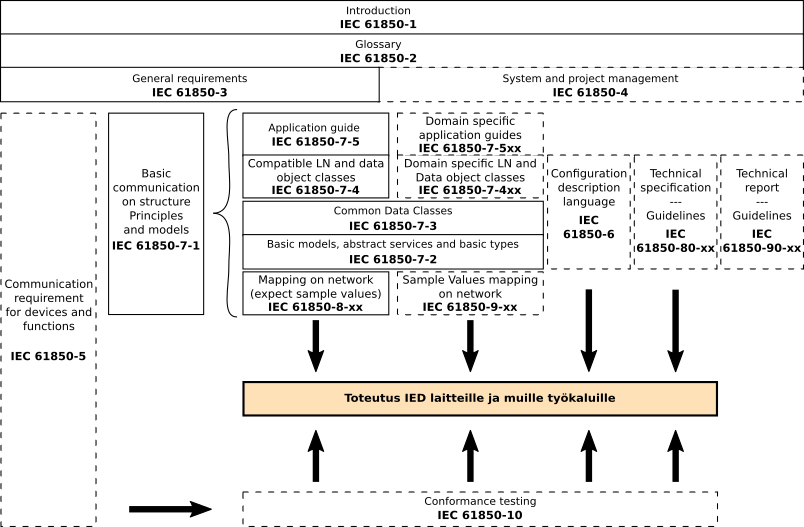
\includegraphics[width=1\textwidth]{pictures/iec61850-series-parts-and-relations.png}
	\caption{IEC 61850 -standardin osat ja niiden väliset relaatiot.}
	\label{fig:iec61850-osat-ja-relaatiot}
\end{figure}

Standardin ensimmäiset osat 1--5 kattavat yleistä kuvaa standardista ja sen vaatimuksista. Osiossa 6 käsitellään IED-laitteiden konfigurointiin käytetty XML (engl. Extensible Markup Language) -pohjainen kieli \cite[s.~7--8]{IEC61850-6}. Tämä osuus ei ole tämän työn kannalta tärkeä ja sitä ei sen tarkemmin käsitellä. Osat 7-1--7-4 käsittelevät standardin abstraktia mallia, niiden palveluita ja kuinka se rakentuu. Abstrahoidut palvelut ja mallit standardissa lyhennetään ACSI (engl. Abstract Communication Service Interface), ja samaa lyhennettä käytetään tässä työssä \cite[s.~72]{IEC61850-7-1}. Osissa 8--9 ja niiden alakohdissa käsitellään abstraktimallien toteuttamista erillisille protokollille, jolloin malleista tulee kyseisestä tekniikasta riippuvaisia. Tässä työssä käytettiin osaa 8-1, joka toteuttaa absrahit mallit MMS-protokollalle. Osa 10 käsittelee testausmenetelmiä, joilla voidaan varmistaa standardin määritysten noudattaminen. Tämä osuus ei myöskään ole tämän työn kannalta tärkeä, ja sitä ei teoriassa sen tarkemmin käsitellä. \cite[s.~15]{IEC61850-7-1}


\subsection{Abstraktimallin käsitteet ja niiden käyttö}
IEC 61850 -standardin lähtökohtana on pilkkoa koko sähköaseman toiminnallisuuden funktiot pieniksi yksilöiksi. Pilkotut yksilöt abstrahoidaan ja pidetään sopivan kokoisina, jotta ne voidaan konfiguroida esitettäväksi erillisellä IED-laiteella. Yksi aseman funktio voidaan hajauttaa monelle eri IED-laitteelle. Esimerkiksi linjan suojaukseen liittyvät komponentit, katkaisija (engl. circuit braker) ja ylivirtasuoja (engl. overcurrent protection). Toimiakseen yhdessä, laitteiden täytyy vaihtaa informaatiota keskenään verkon yli \cite[s.~31]{IEC61850-7-1}. Standardi määrittää seuraavat käsitteet sähköaseman funktioiden mallintamiseen:
\begin{itemize}
	\item fyysinen laite (engl. physical device, lyhennetään PD),
	\item looginen laite (engl. logical device, lyhennetään LD),
	\item looginen noodi (engl. logical node, lyhennetään LN),
	\item dataobjekti (engl. data object, lyhennetään DO),
	\item data-attribuutti (engl. data atribute, lyhennetään DA).
\end{itemize}
Käsiteet muodostavat mallista hiearkisen puurakenteen ja ne on listattu hierarkisessa järjestyksessä. Puun juurena on fyysinen laite, sen alla voi olla yksi tai useampi looginen laite, loogisen laitteen alla yksi tai useampi looginen noodi jne. Käsitteillä standardissa virtualisoidaan aseman funktiot, esimerkiksi suojaus. Kuvassa \ref{fig:substation-abstraction} on esitetty, kuinka sähköaseman fyysiset laitteet voidaan mallintaa standardin määrittämillä käsitteillä. Samaa periaatetta käytetään kaikille aseman laitteille. Kuvassa ensin uloimpana on fyysinen laite, joka ohjaa aseman oikeita laitteita ja tarkkailee niiden toimintaa. Tämä laite voi olla IED-laite, joka on myös samalla kytketty aseman verkkoon ja sillä on IP-osoite. Yksi IED-laite voi olla samaan aikaan kytkettynä aseman moneen muuhun oikeaan laitteeseen. Tämän jälkeen mallinnetaan aseman joukko laitteita loogiseksi laitteeksi. Tällainen voi esimerkiksi olla tietyn jännitetason (engl. bay) komponentit, kuten katkaisijat, muuntajat jne. Kuvassa kaksi muuntajaa on mallinnettu yhdeksi loogiseksi laitteeksi, koska ne kuuluvat samaan jännitetasoon. Looginen laite koostuu loogisista noodeista se mallintaa jotakin aseman ohjattavaa yksittäistä laitetta. Kuvassa kaksi muuntajaa mallinnetaan loogisiksi noodeiksi. Jotta oikeaa fyysistä muuntajaa voidaan kuvata mallilla. Täytyy siitä pystyä esittämään mitattavia tai kuvaavia arvoja, esimerkiksi mitatut jännitteen arvot. Näihin tarkoituksiin käyteään käsitteitä dataobjekti ja data-attribuutti. Looginen noodi koostuu dataobjekteista ja dataobjekti koostuu data-attribuuteista. Data-attribuutti esittää yhtä mitattavaa tai kuvaavaa arvoa laitteesta, esimerkiksi sen hetkinen jännite tai laitteen tila. Dataobjekti on tapa koostaa yhteen kuuluvat data-attribuutit saman käsitteen alle, esimerkiksi mittaukseen tai ohjaukseen liittyvät data-attribuutit. \cite[s.~2]{Camachi2017} \cite[s.~24]{IEC61850-1}

\begin{figure}[ht!]
	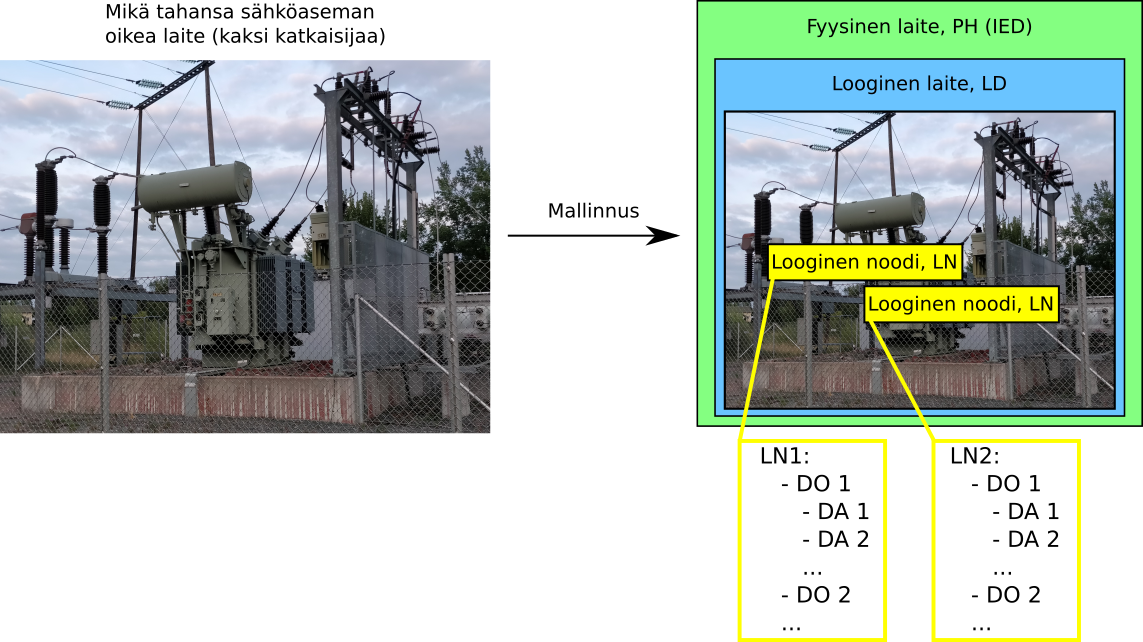
\includegraphics[width=1\textwidth]{pictures/substation-abstraction.png}
	\caption{Sähköaseman fyysisten laiteiden abstrahointi IEC 61850 -standardin käsitteillä (pohjautuu kuvaan \cite[s.~17]{IEC61850-7-1}).}
	\label{fig:substation-abstraction}
\end{figure}

IEC 61850 -standardin käsitteiden avulla sähköaseman laitteet ja funktiot voidaan esittää malleilla. Malleja voidaan käyttää IED-laitteiden konfiguroinnin määrittämiseen ja tietona, jotka voidaan siirtää verkon yli laitteelta toiselle. Jotta käsitteitä voidaan käyttää konfigurointiin ja kommunikointiin, standardi määrittää lisää tarkuutta käsitteisiin ja kuinka niitä käytetään. MMS-protokollan kanssa fyysinen laite yksilöidään IP-osoiteella. Tätä käsitettä ei käytetä kommunikointiin tai konfigurointiin. Fyysisen laitteen käsite on olemassa standardissa, jotta se voidaan pitää abstraktina toteutettavasta tekniikasta. Looginen laite yksilöidään nimellä, joka on yksilöllinen IED-laitteessa. Standardi ei ota kantaa loogisen laitteen nimeämiseen. Looginen noodi yksilöidään IED-laiteella myös nimellä. Looginen noodi esitetään IED-laitteella jonkin standardissa määrittettyjen luokan instanssina. Standardin osassa 7-4 määritetään valmiita luokkia käytettäväksi eri laitteiden esittämiseen. Esimerkiksi katkaija on määritelty luokkaan tyyppiltään XCBR (engl. circuit braker) \cite[s.~105--106]{IEC61850-7-4}. Sähköaseman insinööri, joka konfiguroi IED-laitteen, määrittää konfiguraatiotiedostossa, että kytketty katkaisija esitetään XCBR-luokan instanssina ja nimeää sen standardin ohjeiden mukaan. Näin IED-laite tietää mitä laitetta se esittää ja ohjaa. IED-laitteessa kaikki eri luokkien instanssit yksilöidään nimillä ja niitä käytetään kun olioon viitataan esimerkiksi palvelukutsulla tai konfiguraatiolla. Looginen noodi koostui dataobjekteista. Standardissa dataobjektit on myös määritetty luokkina, joista tehdään instansseja. Erona on, että loogisen noodin luokkan tyyppi määrittää mitä dataobjektin luokkia insansioidaan, ja millä nimellä ne esitettään loogisen noodin instanssissa. Standari määrittää dataobjektien luokkien tyypit standardissa osassa 7-3. Dataobjekti koostuu data-attribuuteista. Kuten loogisen noodin luokan tyyppi, dataobjektin luokka määrittää käytettävät data-attribuutit ja niiden nimet. Tällä kertaa data-attribuutti ei ole välttämättä suoraan ole luokka. Data-attribuutit voivat olla primitiivisiä tyyppejä, kuten integer ja float. Tai ne voivat olla ns. rakennettuja data-attribuutteja (enlg. constructed attribute classes), jotka pitävät sisällään tarkempia data-attribuutteja. Hyvä esimerkki on data attribuutti nimeltään q, jonka tyyppi on Quality. Standardin mukaan tällä tyypillä on vielä aliattribuutteina mm. validity, detailQual jne \cite[s.~11]{IEC61850-7-3}. Standardi ei rajoita sitä, että dataobjektin alla pitää aina data-attribuutteja. Joissakin tapauksissa dataobjektin alla on toinen dataobjekti ja tämän alla vasta data-attribuutit. Kaikkien luokkien tyyppeihin määritetyt kentät ja niiden nimet voi löytyvät standardista. Kappaleessa \ref{ch:luokkien-rakentuminen-instanseista} käydään tarkemmin läpi kuinka luokkien hierarkia standardissa rakentuu. \cite{IEC61850-1, IEC61850-7-1, IEC61850-7-2, IEC61850-7-3}

% TODO: Jatka lukemista tästä!


\subsection{Loogisen noodin luokkien ja attribuuttien rakentuminen}
\label{ch:luokkien-rakentuminen-instanseista}
IEC 61850 -standardissa kaikki luokat määritellään taulukoilla, joissa on standardoitu kentän nimi, tyyppi, selitys ja onko kenttä optionaalinen. Tässä teoriaosuudessa mennään syvemmälle luokkien määritykseen. Ja esitetään esimerkkinä kuinka standardin pohjalta instansioitu looginen noodi ja sen alitason dataobjektit ja data-attribuutit rakentuvat. Esimerkissä käytetään kuvan \ref{fig:iec61850-data-modeling} rakennetta. Nimet ja luokkien instanssit konfiguroidaan IED-laitteelle XML-pohjaisella konfiguraatiotiedostolla. Tämä määritellään standardin osassa 6. Kuvassa \ref{fig:iec61850-data-modeling} fyysinen laite on IED-laite ja siihen verkossa viitataan IP-osoitteella 192.192.1.100. IED-laitteelle on konfiguroitu looginen laite nimeltä MyLD. Eri loogiset laitteet IED-laitteella yksilöi vai sen nimi. Loogisella laitteella on kaksi instanssia loogisen noodin luokista nimillä MMXU1 ja XCBR1. MMXU1 instanssi on tyyppiä MMXU (engl. measurement) \cite[s.~57--58]{IEC61850-7-4} ja XCBR1 on tyyppiä XCBR (engl. circuit breaker). Kyseessä on siis vastaavasti mittaukseen liittyvä laite ja aikaisemmin mainittu linjan katkaisija. XCBR1 loogisella noodilla on dataobjekti nimeltään Pos (engl. position), joka on tyyppiä DPC (engl. controllable double point). Ja MMXU1 nimeltään TotW (engl. total active power), joka on tyyppiä MV (engl. measured value). Loogisilla noodeilla on määritetty enemmänkin dataobjekteja eri nimillä, mutta kuvassa \ref{fig:iec61850-data-modeling} on esitetty vai yhdet yksinkertaisuuden takia. Pos dataobjektilla on data-attribuutit nimeltään stVal, q ja t. Ja TotW dataobjektilla on data-attribuutit mag, q ja t. Esimerkin data-attribuutti q on tyyppiä Quality, jolla on alidata-attribuutteja ja attribuutti StVal on tyyppiä boolean.

\begin{figure}[ht!]
	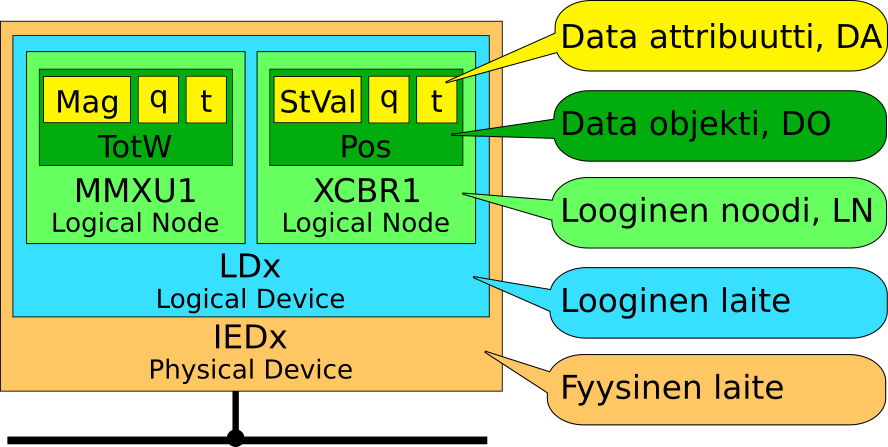
\includegraphics[width=1\textwidth]{pictures/iec61850-data-modeling.png}
	\caption{Standardin käsitteiden hierarkinen rakenne ja niiden nimeämisen esimerkki}
	\label{fig:iec61850-data-modeling}
\end{figure}

Standardissa osassa 7-4 on lista kaikista sen määrittämistä loogisen noodin luokista eri tarkoituksiin. Taulukossa \ref{tab:iec61850-xcbr-class-definition} on esitetty XCBR-luokan määritys. Taulukosta voi nähdä luokan instanssille määritetyt kenttien nimet ja viimeinen sarake M/O/C, kertoo onko kenttä pakollinen (Mandatory, M), optionaalinen (Optional, O), vai konditionaalinen (Conditional, C) \cite[s.~106]{IEC61850-7-4}. Taulukosta voi nähdä kuvan \ref{fig:iec61850-data-modeling} esimerkin XCBR1-instanssin data-objektin nimeltä Pos ja sen tyypin DPC. Standardissa dataobjektien luokkia kutsutaan yleisiksi luokiksi (engl. Common Data Class, lyhennetään CDC). Näin sen takia, koska samaa dataobjektin luokkaa voidan käyttää monessa eri loogisen noodin luokassa. Standardin dataobjektin luokat on tarkoitettu kerätä yhteen samaan asiaan liittyvät data-attribuutit. CDC-luokkien määritykset löytyvät standardin osasta 7-3 \cite[s.~26]{IEC61850-1}. Joillakin CDC-luokkien attribuutteina voi olla vielä muita CDC-luokkia. Tällöin standardissa puhutaan yleisistä aliluokista (engl. sub data object). Esimerkkinä tästä on CDC-luokka WYE, jolla on attribuuttina phsA niminen kenttä, joka on tyyppiä CMV. CMV on CDC-luokka, jolla on taas omat data attribuuttinsa. \cite[s.~51,61]{IEC61850-7-2} \cite[s.~36]{IEC61850-7-3}

\begin{table}[ht!]
	\caption{IEC 61850 -standardin katkaisijaluokan XCBR -määritys.}
	\label{tab:iec61850-xcbr-class-definition}
	\begin{tabular}{l | l | l | l}
		\hline
		\textbf{Data objektin nimi} & \textbf{Englanniksi} & \textbf{CDC-luokka} & \textbf{M/O/C} \\
		\hline \hline
		\multicolumn{4}{l}{\textbf{Selitys}} \\
		\hline
		EEName & External equipment name plate & DPL & O \\
		\hline
		\multicolumn{4}{l}{\textbf{Tila informaatio}} \\
		\hline
		EEHealt & External equipment health & ENS & O \\
		LocKey & Local or remote key & SPS & O \\
		Loc & Local control behaviour & SPS & M \\
		OpCnt & Operation counter & INS & M \\
		CBOpCap & Circuit breaker operating capability & ENS & O \\
		POWCap & Point on wave switching capability & ENS & O \\
		MaxOpCap & Circuit breaker operating capability & INS & O \\
		Dsc & Discrepancy & SPS & O \\
		\hline
		\multicolumn{4}{l}{\textbf{Mitatut arvot}} \\
		\hline
		SumSwARs & Sum of switched amperes, resettable & BRC & O \\
		\hline
		\multicolumn{4}{l}{\textbf{Kontrollit}} \\
		\hline
		LocSta & Switching authority at station level & SPC & O \\
		Pos & Switch position & DPC & M \\
		BlkOpn & Block opening & SPC & M \\
		BlkCls & Block closing & SPC & M \\
		ChaMotEna & Charger motor enabled & SPC & O \\
		\hline
		\multicolumn{4}{l}{\textbf{Asetukset}} \\
		\hline
		CBTmms & Closing time of braker & ING & O \\
		\hline
	\end{tabular}
\end{table}

Taulukossa \ref{tab:iec61850-DPC-class-definition} on esitetty XCBR-luokan Pos-attribuutin, DPC-luokan määritys \cite[s.~44]{IEC61850-7-3}. Taulukosta voi nähdä kuvan \ref{fig:iec61850-data-modeling} esimerkissä esitetyt data-attribuutit stVal, q ja t ja niiden tyypit. Attribuuttien tyyppejä on paljon enemmänkin ja lukija voi tarvittaessa tarkistaa kaikki tyypit standardista. Tällä periaatteella standardi rakentaa kaikki muutkin luokat hierarkisesti ja sen avulla voidaan selvittää mitä dataobjekteja looginen noodi sisältää, mitä data-attribuutteja mikäkin data objekti sisältää. Taulukossa \ref{tab:iec61850-DPC-class-definition} on myös määritetty data-attribuuttien funktionaaliset rajoitteet (engl. Functional Constraint, lyhennetään FC), sekä mahdolliset liipaiseimet (engl. trigger options, lyhennetään TrgOp). Nämä kaksi asiaa käsitellään teoriassa tuonnempana.

\begin{table}[ht!]
	\caption{IEC 61850 -standardin DPC-luokan määritys.}
	\label{tab:iec61850-DPC-class-definition}
	\begin{tabular}{l | l | l | l}
		\hline
		\textbf{Data attribuutin nimi} & \textbf{Tyyppi} & \textbf{FC} & \textbf{Liipaisin (TrgOp)} \\
		\hline
		\multicolumn{4}{l}{\textbf{Tila ja ohjaus}} \\
		\hline
		origin & Originator & ST &  \\
		ctlNum & INT8U & ST &  \\
		stVal & CODEC ENUM & ST & dchg \\
		q & Quality & ST & qchg \\
		t & TimeStamp & ST &  \\
		stSeld & BOOLEAN & ST & dchg \\
		opRcvd & BOOLEAN & OR & dchg \\
		opOk & BOOLEAN & OR & dchg \\
		tOpOk & TimeStamp & OR &  \\
		\hline
		\multicolumn{4}{l}{\textbf{Vaihtoehtoinen ja estäminen}} \\
		\hline
		subEna & BOOLEAN & SV &  \\
		subVal & CODED ENUM & SV &  \\
		subQ & Quality & SV &  \\
		subID & VISIBLE STRING64 & SV &  \\
		blkEna & BOOLEAN & BL &  \\
		\hline
		\multicolumn{4}{l}{\textbf{Asetukset, selitys ja laajennos}} \\
		\hline
		pulseConfig & PulseConfig & CF & dchg \\
		ctlModel & CtlModels & CF & dchg \\
		sboTimeOut & INT32U & CF & dchg \\
		sboClass & SboClassses & CF & dchg \\
		operTimeout & INT32U & CF & dchg \\
		d & VISIBLE STRING255 & DC &  \\
		dU & UNICODE STRING255 & DC &  \\
		cdcNs & VISIBLE STRING255 & EX &  \\
		cdcName & VISIBLE STRING255 & EX &  \\
		dataNs & VISIBLE STRING255 & EX &  \\
		\hline
	\end{tabular}
\end{table}

Kaikkien yllämainittujen luokkien kenttien määritysten lisäksi standardi määrittää palveluita jokaiselle luokkatyypille erikseen. Määritetyt palvelut ovat abstrakteja ja ne toteutetaan tekniikalle erillisellä standardin osalla. Palveluita voi ajatella esimerkiksi suoritettavina funktioina. Esimerkkinä palveluista kaikille dataobjekteille on mm. GetDataValues, joka palauttaa kaikki dataobjektin attribuuttien arvot. SetDataValues kirjoittaa annetut data-attribuuttien arvot. Ja GetDataDirectory palauttaa kaikki data-attribuuttien viitteet kyseisessä dataobjekstissa. Näitä ja muita abstrahoituja malleja viitataan standardissa lyhentellä ACSI (engl. abstract communication service interface) \cite[s.~15,45--46]{IEC61850-7-2} \cite[s.~26]{IEC61850-7-1}.


\subsection{Attribuuttien viittaus hierarkiassa}
IEC 61850 -standardi määrittää erilaisia palvelukutsuja eri luokkatyypeille. Jotta kutsuja voitaisiin tehdä verkon yli IED-laitteelle ja sen arvoja lukea ja asettaa hierarkiassa. Pitää tiettyyn data-attribuuttiin tai data-objektiin voida viitata yksilöivästi. Siksipä standarissa on määritetty viittausformaatti, jota käytetään kun IED-laitteelle kutsuja tehdään. Kutsussa olevan viitteen perusteella IED-laite tietää, mihin instanssiin kutsu kohdistuu ja pystyy toimimaan sen mukaan. Tärkeää on myös mainita, että määritettyjä kutsuja lukemiseen ja asettamiseen voidaan käyttää useaan data-attribuuttiin yhtä aikaa. Kutsuja ei ole rajoitettu käsittelemään yhtä data-attribuuttia kerrallaan. Viitten lisäksi aikaisemmin mainittu funktionaalinen rajoite, kertoo mihin data-attribuutteihin kutsu kohdistuu. Tämä tullaan käsittelemään tarkemmin kappaleessa \ref{ch:fc-and-dataset}. Kuvassa \ref{fig:iec61850-data-reference} on esitetty kuinka standardi määrittää viitteen muodostumisen loogisesta laitteesta data attribuuttiin asti. Viite alkaa loogisen laitteen nimestä ja ei sisällä fyysistä laitetta. Tähän on syynä se, että fyysisellä laitteella ei ole nimeä ja sillä on yksilöivä IP-osoite MMS-protokollan tapauksessa. Fyysinen laite on standardissa abstraktio laitteesta, kuten IED:stä. \cite[s.~93]{IEC61850-7-1}.

\begin{figure}[ht!]
	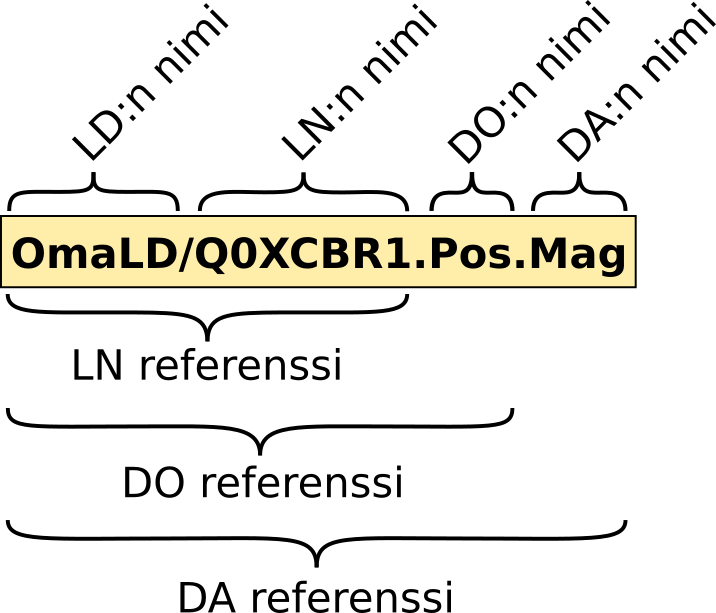
\includegraphics[width=0.5\textwidth]{pictures/iec61850-data-reference.png}
	\caption{IEC 61850 -standardin määrittämä viitteen rakenne.}
	\label{fig:iec61850-data-reference}
\end{figure}

Viite muodostuu suoraan laitteessa olevien luokkien instanssien nimien ja hierarkian mukaan. Loogisen laitteen (LD) ja loogisen noodin (LN) erottimena käytetään kauttaviivaa, ja muiden osien erottimena käytetään pistettä. Loogisella laitteella on aseman insinöörin määrittämä oma nimi, mutta kuitenkin alle 65 merkkiä. Muuten loogisen laitteen nimeen standardi ei puutu. Loogisen noodin instanssin nimi koostuu alku-, keski- ja loppuosasta. Alkuosan käyttäjä voi itse päättää, kuvassa \ref{fig:iec61850-data-reference} Q0. Voi sisältää numeroita ja kirjaimia, mutta täytyy alkaa kirjaimella. Keskiosan täytyy olla loogisen luokan nimi, josta instanssi on tehty. Tässä tapauksessa jo aikaisemmin mainittu katkaisijan luokka, XCBR. Tämä osuus on aina 4 kirjainta pitkä ja on aina isoilla kirjaimilla. Loppuosa on instanssin numeerinen arvo, joka ei sisällä kirjaimia. Loppuosan käyttäjä voi itse päättää, jonka ei tarvitse välttämättä olla juokseva numero. Alku- ja loppuosan yhteenlaskettu merkkien pituus täytyy olla alle 13 merkkiä, eli koko loogisen noodin nimen pituus voi olla maksimissaa 17 merkkiä. Data objektien (DO) ja attribuuttien (DA) niminä käytetään standardin määrittämiä nimiä, jotka määritetään niitä vastaavissa luokissa osissa 7-3 ja 7-4 (katso taulukkot \ref{tab:iec61850-xcbr-class-definition} ja \ref{tab:iec61850-DPC-class-definition}). Riippuen viittauksesta, näistä muodostuu loogisen noodin viite, dataobjektin viite ja data attribuutin viite. Jos data-objektin alla on toinen dataobjekti, jonka alla on vasta itse data-attribuutit. Viittausta vain jatketaan instanssien nimiä liittämällä toisiinsa pisteellä aina data-attribuuttiin asti. Samoin toimitaan kun data-attribuutti on tyypiltään rakennettu tyyppi, kuten Quality, jolla on alidata-attribuutteja. \cite[s.~181--182]{IEC61850-7-2} \cite[s.~93--95]{IEC61850-7-1}

Standardissa määritetään kaksi näkyvyysaluetta (engl. scope) viittaukselle, jotka ovat palvelin- ja looginen laite -näkyvyysalueet. Palvelin tässä yhteydessä tarkoittaa verkkoon kytkettyä laitetta, eli IED-laitetta. Palvelinnäkyvyysalueelle viitataan ottamalla viittauksesta pois loogisen laitteen nimi. Eli kuvassa \ref{fig:iec61850-data-reference} viittaus tulisi muotoon /Q0XCBR1.Pos.stVal. Edellemainittua viittausta käytetään silloin, kun loogisen noodin instanssi sijaitsee loogisen laitteen ulkopuolella, mutta kuitenkin palvelimella. Looginen laite -näkyvyysalueessa viittaus sisältää loogisen laitteen nimen ennen kauttaviivaa, toisin kuin palvelin-näkyvyysalueessa. Esimerkiksi kuvassa \ref{fig:iec61850-data-reference} oleva viittaus OmaLD/Q0XCBR1.Pos.stVal. Loogisen laitteen -näkyvyysaluetta käytetään silloin kun loogisen noodin instanssi sijaitsee loogisen laitteen sisällä sen hierarkiassa. Tässä työssä jatkossa käytetään pelkästään loogisen laitteen -näkyvyysaluetta. \cite[s.~183]{IEC61850-7-2}

Standardi määrittä maksimipituuksia viittauksille. Seuraavaksi kerrotut pituusmääritykset ovat voimassa kummallekin edelle mainitulle näkyvyysalueen viittaukselle. Ennen kauttaviivaa saa olla maksimissaan 64 merkkiä. Tämän jälkeen kauttaviiva, josta seuraa uudelleen maksimissaan 64 merkkiä. Eli koko viittauksen maksimipituus saa olla enintään 129 merkkiä, kauttaviiva mukaan lukien. \cite[s.~24,183]{IEC61850-7-2}


\subsection{Attribuuttien funktionaalinen rajoite ja niistä muodostetut datajoukot}
\label{ch:fc-and-dataset}
Standardin CDC-luokat, määrittävät käytettävät data-attribuutit (katso taulukko \ref{tab:iec61850-DPC-class-definition}). Nämä luokat määrittävät myös jokaiselle data-attribuutille aikaisemmin mainitun funktionaalisen rajoitteen (engl. functional constraint, lyhennetään FC). Funktionaalinen rajoite kuvaa attribuutin käyttötarkoitusta ja sitä mitä palveluita attribuuttiin voidaan käyttää. Esimerkiksi kaikki attribuutit, jotka liittyvät laitteen tilaan (engl. status), niillä on funktionaalinen rajoite ST (standardissa engl. status information). Standardi määrittää paljon erilaisia funktionaalisia rajoitteita, jotka ovat kaikki kahden ison kirjaimen yhdistelmiä. Taulukossa \ref{tab:iec61850-functional-constraints} on esitetty joitain tärkeimpiä funktionaalisia rajoitteita. Funktionaalinen rajoite määrittä myös, onko attribuutti kirjoitettava tai luettava \cite[s.~54]{IEC61850-7-2}.

\begin{table}[ht!]
	\caption{Osa IEC 61850 -standardin määrittämistä funktionaalisista rajoitteitteista (FC).}
	\label{tab:iec61850-functional-constraints}
	\begin{tabular}{l | l | l | l}
		\hline
		\textbf{Lyhenne} & \textbf{Selite} & \textbf{Luettava} & \textbf{Kirjoitettava} \\
		\hline \hline
		ST & Laitteen tilatieto (status) & Kyllä & Ei \\
		MX & Mittaustieto (measurands) & Kyllä & Ei \\
		CF & Laitteen asetusarvo (configuration) & Kyllä & Kyllä \\
		DC & Selitystieto (description) & Kyllä & Kyllä \\
		\hline
	\end{tabular}
\end{table}

Funktionaalista rajoitetta käytetään IED-laitteelle tehtävässä kutsussa viitteen kanssa suodattamaan mitä data-attribuutteja tehty kutsu koskee. Funktionaalinen rajoite on pakollinen tieto kutsuissa, jotka lukevat tai kirjoittavat arvoja. Seuraavaksi esitetään esimerkki kuinka yhdellä kutsulla viitataan moneen data-attribuuttiin. Esimerkkinä otetaan kuvassa \ref{fig:iec61850-data-reference} olevasta viitteestä osa, joka viittaa data-objektiin. Eli OmaLD/Q0XCBR1.Pos, jolloin viite on DO-viite. Kutsun vaikutusalue on aina hierarkiassa alaspäin. Eli nyt viitteellä viitataan Pos-dataobjektin kaikkiin alla oleviin data-attribuutteihin. Katso taulukko \ref{tab:iec61850-DPC-class-definition}, jossa on esitetty kaikki Pos-dataobjektin alla olevat data-attribuutit, johon nyt viitataan. Huomiona, jos viittauksen alla olisi alidata-objekteja, niidenkin data-attribuutit kuuluvat viittauksen piiriin. Viittauksen vaikutuksen voi siis ajatella jatkuvan viittauskohdasta alaspäin rekursiivisesti kaikkiin ali-instansseihin. Funktionaalista rajoitetta käytetään suodattamaan kaikista viitatuista data-attribuuteista ne, jotka halutaan kirjoittaa tai lukea. Esimerkkinä jos kutsuun viitteellä OmaLD/Q0XCBR1.Pos lisättäisiin funktionaalinen rajoite ST. Rajoitettaisiin kutsu koskemaan Pos-dataobjektin alidata-attribuuteista vain niitä attribuutteja, joilla on funktionaalinen rajoite ST. Eli taulukon \ref{tab:iec61850-DPC-class-definition} mukaan attribuutit olisivat origin, ctlNum, stVal, q, t ja stSeld. Muut data-attribuutit suodatetaan pois kutsun vaikutuksesta. Sama suodatus tapahtuu rekursiivisesti hierarkiassa alaspäin kaikille alidata-attribuuteille. Esimerkissä olevat arvot voisi vain lukea, ei kirjoittaa. Tämä sen takia koska taulukon \ref{tab:iec61850-functional-constraints} mukaan funktionaalinen rajoite ST sallii vain lukemisen. IEC 61850 -standardissa määritetään funktionaalinen rajoite XX, joka on sama kuin mikä tahansa muu funktionaalinen rajoite. Kuitenkin standardin osassa 8-1 joka tekee toteutuksen MMS-protokollalle, tämä ei ole tuettu toiminnalisuus. Eli toisin sanoen, jos MMS-protokollan kanssa halutaan lukea kaikki yhden data-objektin data-attribuutit. Joudutaan tekemään kutsu jokaista data-objektin funktionaalista rajoitetta kohti.

Viittauksen ja funktionaalisen rajoitteen avulla siis suodatetaan rekursiivisesti hierarkiassa alaspäin olevia data-attribuutteja. IEC 61850 -standardissa on määritelty nimitykset käytettäväksi kun jotakin viittausta suodatetaan funktionaalisella rajoitteella. Nämä ovat FCD (engl. functional constrained data) ja FCDA (engl. functional constrained data attribute). Nämä nimitykset ovat standardissa vain käsite, joka ei toteudu mitenkään tekniikalla. Taulukossa \ref{tab:fcd-ja-fcda} on esitetty viittauksia eri tyyppisiin instansseihin funktionaalisella rajoitteella. Taulukosta selviää viitattu instanssi dataobjekti (DO) tai data-attribuutti (DA), instanssin tyyppi ja käytetty nimitys viittaukselle FCD tai FCDA. FCD nimitys on silloin kun vain hierarkian ensimmäistä dataobjekti rajoitetaan funktionaalisesti. FCDA nimitys on käytössä kaikille muille viittauksille hierarkiassa alaspäin, joita rajoitetaan funktionaalisesti. Huomaa taulukossa \ref{tab:fcd-ja-fcda} viittaus OmaLD/MMXU1.PhV.phsA, joka viittaa PhV dataobjekin alidataobjektiin. Tämä on FCDA-viittaus, vaikka kyseessä onkin dataobjekti. Ainoa ero FCD:n ja FCDA:n nimitysten välillä on vain se, että FCD-viittaus on aina vain hierarkian ensimmäiseen dataobjektiin ja FCDA-viittaus siitä eteenpäin hierarkiassa. Riippumatta mitä tyyppejä viitatut instanssit hierarkiassa alaspäin ovat. \cite[s.~55]{IEC61850-7-2} \cite[s.~63]{IEC61850-8-1}

\begin{table}[ht!]
	\caption{Viitteen nimeäminen lyhenteellä funktionaalisen rajoitteen kanssa.}
	\label{tab:fcd-ja-fcda}
	\begin{tabular}{l | l | l | l | l}
		\hline
		\textbf{FC} & \textbf{Viite} & \textbf{Instanssi} & \textbf{Tyyppi} & \textbf{Nimitys} \\
		\hline \hline
		ST & OmaLD/XCBR1.Pos & DO & DPC & FCD \\
		ST & OmaLD/XCBR1.Pos.t & DA & TimeStamp & FCDA \\
		ST & OmaLD/XCBR1.Pos.ctlNum & DA & INT8U & FCDA \\
		MX & OmaLD/MMXU1.PhV & DO & WYE & FCD \\
		MX & OmaLD/MMXU1.PhV.phsA & DO & CMV & FCDA \\
		MX & OmaLD/MMXU1.PhV.phsA.t & DA & TimeStamp & FCDA \\
		\hline
	\end{tabular}
\end{table}

Funktionaalista rajoitetta käytetään viitteen kanssa suodattamaan viitatusta kohdasta alaspäin kaikki data-attribuutit. Tätä toiminnallisuutta käytetään hyväksi, kun tehdään kirjoittavia tai lukevia kutsuja ja rajoitetaan kutsulla vaikutettavia data-attribuutteja. Tätä samaa mekanismia käytetään hyväksi kun IED-laitteeseen määritellään datajoukkoja. IEC 61850 -standardissa datajoukko koostuu joukosta IED-laitteessa olemassa olevista data-attribuuteista. Datajoukko on tapa koostaa yhteen kiinnostavat data-attribuutit IED-laitteelta. Datajoukko nimetään ja sijoitetaan IED-laitteen hierarkiaan. Näin siihen voidaan viitata kutsuilla kuten mihin tahansa muuhun hierarkian instanssiin. Datajoukot IED-laitteelle rakennetaan käyttämällä FCD ja FCDA viitteitä. Datajoukko koostuu siis joukosta FCD- ja FCDA -viitteitä. Jokaisella viitteellä on jokin funktionaalinen rajoite, joka suodattaa viitteen alla olevat attribuutit ja sisällyttää ne kyseiseen datajoukkoon. Esimerkkinä datajoukon rakentamisesta taulukon \ref{tab:fcd-ja-fcda} viittet. Näistä viitteistä voitaisiin rakentaa oikea standardin mukainen datajoukko, nimetä se nimellä Testi1, ja lisätä IED-laitteen hiearkiaan kohtaan OmaLD/LLN0.Testi1. Nyt datajoukkoon voisi viitata ja vaikka lukea kaikki sen arvot yhdellä kertaa. Jotta datajoukko saadaan näin tehtyä, tieto tästä pitäisi lisätä IED-laitteen asetustiedostoon. Datajoukkoja IED-laitteessa käytetään muodostamaan joukkoja tärkeistä data attribuuteista, joita voidaan esimerkiksi lukea ja kirjoittaa yhdellä kutsulla. Datajoukkoja käytetään myös tilattavien viestien sisältönä. Viestejä voi standardin mukaan tilata vain datajoukoista olevista data-attribuuteista. \cite[s.~61--68]{IEC61850-7-2}


\subsection{Viestien tilaus ja tilauksen konfigurointi}
\label{ch:viestien-tilaus-ja-tilauksen-konfigurointi}
IEC 61850 -standardi määrittää, kuinka IED-laitteen ulkopuolinen ohjelma voi tilata kiinnostavien data-attribuuttien arvoja verkon yli. Viesti voidaan esimerkiksi lähettää tilaajelle, kun mitatun jännitteen arvo muuttuu. Kyseessä on tilaaja-julkaisija arkkitehtuurimalli, jossa ulkopuolinen ohjelma on tilaaja ja IED-laite julkaisuja. Standardi määrittää, että viestejä voidaan tilata vain datajoukoissa viitatuilla data-attribuuteilta. Milloin viestin lähetys tilaajalle tapahtuu, riippuu siitä kuinka tilaaja liipaisimet asettaa tilauksen yhteydessä. Standardissa määritellään käytettäväksi erilaisia liipaisimia joilla tilaaja voi muokata millä muutoksella viesti pitäisi lähettää. Standardissa on myös määritetty mekanismit, jolla tilajaa voi pyytää kaikki arvot kerralla tai tilata jaksottaisia viestejä tietyn aikavälein.

Standardissa määritetään luokka, jonka tehtävä on hoitaa tilausta ja sen asetuksia. Tässä kappaleessa käydään läpi luokan yleistä toiminnallisuutta, kappaleessa \ref{rcb-toiminta} käsitellään luokan attribuutteja ja toimintaa syvällisemmin. Niinkuin muutkin luokat standardissa, tästä tehdään instanssi, sille annetaan yksilöivä nimi ja se lisätään IED-laitteen hierarkiaan. Nämä määritellään IED-laitteen asetustiedostossa, kuten kaikki muutkin instanssit. Yksilöivän nimen avulla tilaaja voi viitata kutsulla instanssiin, muuttaa luokan asetuksia ja aloittaa tilauksen. Nämä luokat standardissa ovat puskuroitu viestintäluokka (engl. Buffered Report Control Block, lyhennetään BRCB) ja ei puskuroitu luokka (engl. Unbuffered Report Control Block, lyhennetään URCB). Tekstissä kumpaakin luokkaan viitatessa käytetään lyhennettä RCB. Ainoa ero luokkien toiminnan välillä on, että BRCB puskuroi viestejä jonkin aikaa yhteyden katkettua. Yhteyden palautuessa, se lähettää puskuroidut viestit järjestyksessä asiakkaalle. BRCB takaa viestien järjestyksen ja saatavuuden. URCB lähettää viestejä asiakkaalle ilman puskurointia ja yhteyden katketessa, viestit menetetään. Standardissa määritetään, että yksi RCB-instanssi voi palvella vain yhtä tilaaja kerrallaan. Eli IED-laitteeseen täytyy määrittää instansseja sen tilaajien määrän mukaan.

Kuvassa \ref{fig:iec61850-brcb-communication} on esitetty tilaajan ja IED-laitteen välinen viestien tilauksen prosessi. Kuvassa ensin asiakas tilaa puskuroidun BRCB-instanssin. Ensimmäisessä kutsussa tilaaja kirjoittaa RCB-luokan arvot, kuten käytettävät liipaisimet jne. Kutsussa tilaajan on merkittävä RCB-instanssin varatuksi, jotta tilaus käynnistyy. IED-laite aloittaa viestien julkaisun tilaajalle määritettyjen ehtojen mukaan. Jos tilaaja ja IED-laitteen välinen yhteys katkeaa, BRCB-intanssi puskuroi viestejä johonkin järkevään rajaan asti. Kun yhteys tilaajan palaa, IED lähettää viestit järjestyksessä tilaajalle alkaen ensin puskurista. Tilaaja voi lopettaa tilauksen ja instanssin varauksen merkitsemällä sen taas vapaaksi.

\begin{figure}[ht!]
	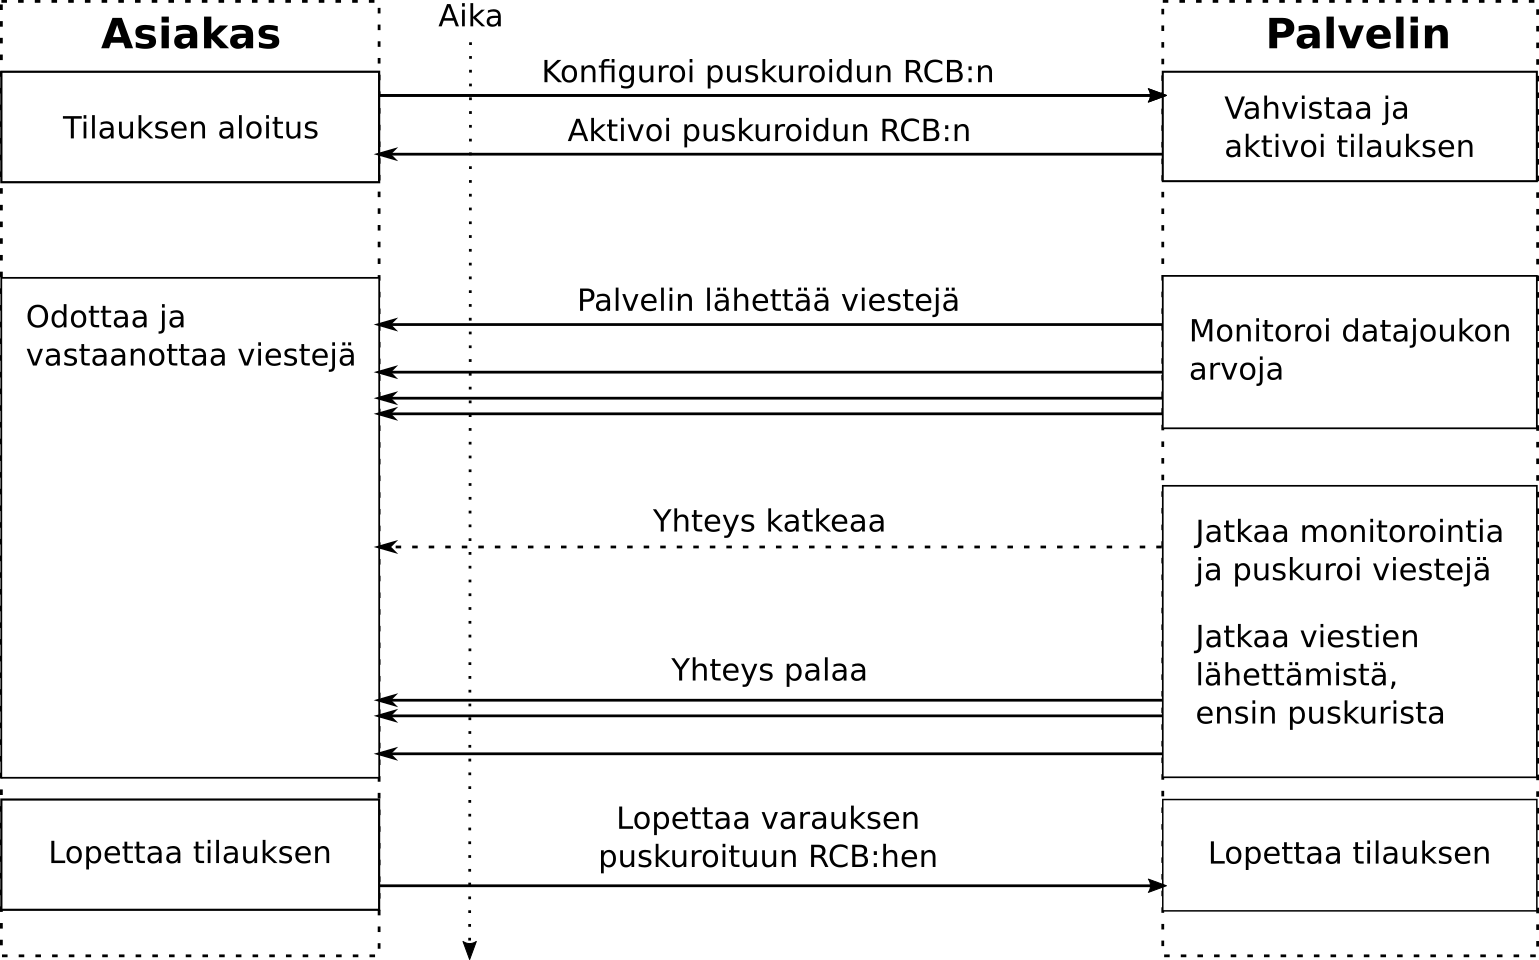
\includegraphics[width=1\textwidth]{pictures/iec61850-brcb-communication.png}
	\caption{Puskuroitu viestien tilausprosessi tilaajan ja IED-laitteen välillä.}
	\label{fig:iec61850-brcb-communication}
\end{figure}

Standardissa määritetään, että viestejä voidaan tilata vain datajoukoista. IED-laitteen asetustiedostossa täytyy myös määrittää mitä datajoukkoa RCB-intanssi käyttää. Tämän jälkeen instanssi tarkkailee datajoukkon attribuuttien muutoksia ja lähettää viestin, jos tilaajan asettama liipaisin täsmää. Koska yksi RCB voi palvella vai yhtä tilaajaa kerrallaan, täytyy samaan datajoukkoon viitata monella eri RCB-instanssilla. Näin monta eri tulevat tilaajaa saamaan viestin samasta tapahtumasta.

Standardissa on määritetty seuraavat liipaisimet data-attribuuteille, joita RCB tarkkailee ja reagoi niihin:
\begin{itemize}
	\item datan muutos (engl. data change, standardissa lyhenne dchg),
	\item laadun muutos (engl. quality change, standardissa lyhenne qchg), ja
	\item datan päivitys (engl. data update, standardissa lyhenne dupd).
\end{itemize}
Jokaiselle data-attribuutille määritellään erikseen mitä liipaisimia se tukee. Nämä määritellään standardin luokkien määrityksissä. Esimerkkinä aikaisemmin mainittu DPC-luokan määritys taulukossa \ref{tab:iec61850-DPC-class-definition}, jossa TrgOp-sarake kertoo attribuutin liipaisimen. Data muutos ja päivitys liipaisimen ero on, että datan päivitys liipaisee tapahtuman, vaikka attribuutin uusi arvo olisi sama. Datan muutos ei liipaise tapahtumaa, jos uusi arvo on sama kuin edellinen arvo. Laadun muutos liipaisin tarkoittaa, että data attribuuttiin liitetty laatuarvo muuttui. Laatuarvo kertoo tilaajalle ja arvojen lukijalle, voiko attribuutien arvoihin luottaa. Laatuarvo on tyyppiä Quality ja tästä voi tarvittaessa lukea enemmän standardista. \cite[s.~90]{IEC61850-7-1}


\subsection{Raportointi-luokan määritys ja toiminta}
\label{rcb-toiminta}
BRCB-luokalla on erilaisia attribuutteja, joita tilaaja voi kirjoittaa ja lukea ennen tilauksen aloittamista. BRCB ja URCB -luokat eivät eroa paljon attribuuteilla toisistaan, joten tässä kappaleessa keskitytään vain BRCB-luokan toimintaan. Tarkka määritys luokkien eroista löytyy standardin osasta 7-2. Taulukossa \ref{tab:iec61850-brcb-class-definition} on esitetty standardin määrittämän BRCB-luokan attribuutit, attribuutin nimi englanniksi ja sen selite. Taulukossa ei ole esitetty attribuuttien tyyppejä, koska ne voi lukija tarvittaessa tarkemmin lukea standardin omasta määrityksestä. Lisäksi tässä kappaleessa käydään läpi luokan atrribuuttien toiminta pääpiirteittäin ja loput tiedot lukija voi tarkistaa standardista. \cite[s.~93--118]{IEC61850-7-2}.

\begin{table}[ht!]
	\caption{BRCB-luokan määritetyt attribuutit ja niiden selitteet.}
	\label{tab:iec61850-brcb-class-definition}
	\begin{tabular}{l | l | l}
		\hline
		\textbf{Attribuutti} & \textbf{Englanniksi} & \textbf{Selite} \\
		\hline \hline
		BRCBName & BRCB name & Objektin nimi \\
		BRCBRef & BRCB reference & Objektin viite \\
		RptID & Report identifier & \parbox[t]{7.5cm}{RCB-instanssin yksilöivä id lähetettyihin viesteihin, asiakas voi asettaa} \\
		RptEna & Report enable & Varaa RCB:n ja aloittaa viestien lähetyksen \\
		DatSet & Data set reference & Tarkailtavan datajoukon viite \\
		ConfRev & Configuration revision & \parbox[t]{7.5cm}{Juokseva konfiguraation numerointi, muutos kasvattaa numerointia} \\
		OptFlds & Optional fields & Mitä optionaalisia kenttiä viestiin lisätään \\
		BufTm & Buffer time & \parbox[t]{7.5cm}{Puskurointiaika, ennen viestin lähetystä. Tänä aikana tapahtuvat liipaisut yhdistetään samaan viestiin} \\
		SqNum & Sequence number & Juokseva lähetetyn viestin numerointi \\
		TrgOps & Trigger options & Millä liipaisimilla viesti lähetetään \\
		IntgPd & Integrity period & \parbox[t]{7.5cm}{Periodisen viestien väli millisekunteina, arvolla 0 ei käytössä} \\
		GI & General-interrogation & \parbox[t]{7.5cm}{Käynnistää yleiskyselyn, joka sisältää kaikki datajoukon attribuutit seuraavaan viestiin} \\
		PurgeBuf & Purge buffer & Puhdistaa lähettämättömät viestit puskurista \\
		EntryID & Entry identifier & \parbox[t]{7.5cm}{Puskurissa olevan viimeisimmän viestin id. Arvo 0 tarkoittaa tyhjää puskuria} \\
		TimeOfEntry & Time of entry & \parbox[t]{7.5cm}{Puskurissa olevan viimeisimmän viestin aikaleima} \\
		ResvTms & Reservation time & \parbox[t]{7.5cm}{Instanssin varausaika sekunteina kun yhteys katkeaa, arvo -1 tarkoittaa konfiguraation aikaista varausta ja 0 että ei varausta} \\
		Owner & Owner & \parbox[t]{7.5cm}{Yksilöi varaavan asiakkaan, yleensä IP-osoite tai IED-laitteen nimi. Arvo 0 että RCB on vapaa tai ei omistajaa} \\
		\hline
	\end{tabular}
\end{table}

Tilaaja voi vapaasti RCB-instanssin arvoja kirjoittaa ja lukea ennen tilauksen aloittamista monella peräkkäisellä kutsulla. Tärkein attribuutti luokassa on RptEna, joka on boolean tyyppiä. Kun attribuutti kirjoitetaan arvoon tosi, aloittaa instanssi tilauksen ja varaa sen tilaajalle. Tilauksen olleassa päällä, tilaaja voi edelleen lukea ja kirjoittaa sen arvoja, mutta rajoitetusti. Joidenkin arvojen kirjoitus pitää tapahtua ennen tilausta tai samassa kutsussa kun RtpEna laitetaan arvoon tosi. Tilaaja lopettaa tilauksen, jos yhteys on poikki tarpeeksi kauan tai RptEna kirjotetaan arvoon epätosi.

RCB-luokan TrgOps-attribuutti on binääritietue, jossa yksittäinen bitti ilmaisee mikä liipaisin aiheuttaa viestin lähettämisen. Tällä attribuutilla tilaaja voi päättää mitä liipaisimia haluaa käyttää. TrgOps sisältää seuraavat liipaisimet:
\begin{itemize}
	\item datan muutos (engl. data change, standardissa lyhenne dchg),
	\item laadun muutos (engl. quality change, standardissa lyhenne qchg), ja
	\item datan päivitys (engl. data update, standardissa lyhenne dupd),
	\item yleinen kysely (enlg. general-interrogation, standardissa lyhenne GI), ja 
	\item jatkuva viestintä väliajoin (engl. intergrity).
\end{itemize}

Kolme ensimmäistä liipaisinta dchg, qchg ja dupd ovat aikaisemmin kappaleessa \ref{ch:viestien-tilaus-ja-tilauksen-konfigurointi} määrittettyjen data attribuuttien liipaisimia. Asiakas voi tilata viestejä esimerkiksi vain datan muutoksista ja ei muista. RCB-luokka määrittää data attribuuttien liipaisimien lisäksi vielä kaksi liipaisinta lisää, yleinen kysely ja jatkuva viestintä väliajoin. Yleinen kysely on viesti, johon RCB sisällyttää kaikki datajoukon attribuutit. Ja jonka asiakas voi liipaista asettamalla luokan attribuutin GI arvoksi tosi ja TrgOps attribuutissa liipaisin on päällä. Tällöin RCB käynnistää viestin generoinnin ja lähettää sen asiakkaalle. Jos liipaisin ei ole päällä TrgOps attribuutissa, ja GI arvoksi asetetaan tosi. RCB ei generoi viestiä. Viestin lähetyksen jälkeen RCB itse asettaa GI:n arvoksi epätosi. Jatkuva viestintä liipaisin on jatkuvaa viestin lähettämistä tilaajalle väliajoin, johon sisältyy kaikki datajoukon attribuutit, kuten yleisessä kyselyssä. Toiminnon saa päälle kun asiakas asettaa RCB-luokassa attribuutit IntgPd arvoksi muu kuin 0, ja TrgOps-attribuutin arvossa kyseinen liipaisin on päällä. Attribuutti IntgPd kertoo minkä väliajoin viesti generoidaan ja lähetetään asiakkaalle. Jos IntgPd arvo on muu kuin 0 ja TrgOps attribuutissa liipaisin ei ole päällä, ei viestiä generoida ja lähetetä asiakkaalle väliajoin.

RCB-luokan attribuuttin OptFlds avulla asiakas voi asettaa mitä vaihtoehtoisia kenttiä viestiin sisällytetään. Attribuutin OptFlds on binääritietue, niin kuin ja TrgOps, ja taulukossa \ref{tab:iec61850-optional-fields-definition} on esitetty sen asetettavat arvot \cite[s.~98]{IEC61850-7-2}. Taulukon yksittäinen kenttä vastaa OptFlds arvon yhtä bittiä. Missä järjestyksessä bitit ovat, määräytyy standardin toteutuksesta tekniikalle, kuten MMS-protokollalle. Taulukon arvoilla tilaaja voi määrittää mitä lisätietoa viestiin sisällytetään. Esimerkiksi asettamalla reason-for-inclusion bitin päälle, liitetään viestin arvon yhteyteen miksi tämä arvo viestiin sisällytettiin. Viestin rakennetta ja kuinka OptFlds-attribuutin arvoilla sen sisältöön voi vaikuttaa käydään läpi tarkemmin kappaleessa \ref{ch:viestin-rakenne}.

\begin{table}[ht!]
	\caption{RCB-luokan OptFlds-attribuutin arvot ja niiden selitteet.}
	\label{tab:iec61850-optional-fields-definition}
	\begin{tabular}{l | l}
		\hline
		\textbf{Arvo} & \textbf{Selite} \\
		\hline \hline
		sequence-number & Jos tosi, sisällytä RCB-luokan attribuutti SqNum viestiin \\
		report-time-stamp & Jos tosi, sisällytä RCB-luokan attribuutti TimeOfEntry viestiin \\
		reason-for-inclusion & Jos tosi, sisällytä syy miksi arvo(t) sisällytettiin viestiin \\
		data-set-name & Jos tosi, sisällytä RCB-luokan attribuutti DatSet viestiin \\
		data-reference & \parbox[t]{10cm}{Jos tosi, sisällytä datajoukon liipaisseen kohdan rakentamiseen käytetty FCD- tai FCDA-viite viestiin} \\
		buffer-overflow & \parbox[t]{10cm}{Jos tosi, sisällytä viestiin tieto onko puskuri vuotanut yli kentällä BufOvfl (engl. buffer overflow)} \\
		entryID & Jos tosi, sisällytä RCB-luokan attribuutti EntryID viestiin \\
		conf-revision & Jos tosi, sisällytä RCB-luokan attribuutti ConfRev viestiin \\
		\hline
	\end{tabular}
\end{table}

Lähetetyt viestit voivat sisältää vaihtelevan määrän sisällytettyjä arvoja. RCB-instanssi mittaa aikaa ensimmäisestä liipaisusta sen attribuutin BufTm verran ja tämän ajan jälkeen pakkaa kaikki liipaisseet attribuutit samaan viestiin. Tilaaja voi muuttaa arvoa jos haluaa käyttää pitempää tai lyhyempää puskurointiaikaa.


\subsection{Viestin rakenne ja kuinka sen sisältö muodostuu}
\label{ch:viestin-rakenne}
IED:n lähettämä viesti on rakenteeltaan hiukan monimutkainen ja lisäksi siihen vaikuttaa RCB-instanssin OptFlds-attribuutin asetetut bitit (taulukko \ref{tab:iec61850-optional-fields-definition}). Tässä kappaleessa käsitellään viestin mallia, joka on tekniikasta riippumaton. Minkälainen viestin rakenne on MMS-protokollan tasolla, siitä ei tarvitse välittää. Toteutetussa ohjelmassa käytettiin kirjastoa, joka hoitaa matalan tason asiat ja tarjoaa helppokäyttöisen rajapinnan viestin sisältöön. Kuitenkin viestin rakenteesta täytyy ymmärtää kuinka vaihtoehtoiset kentät siihen vaikuttavat ja kuinka attribuuttien arvot viestiin sisällytetään. Kuvassa \ref{fig:iec61850-report-format} on esitetty standardin määrittämän viestin rakenne ja mitä kenttiä OptFlds-attribuutti kontrolloi. Viestin rakenteen voisi ajatella koostuvan kahdesta osasta. Ensin viestissä on yleinen tieto ja viimeisenä taulukko datajoukon alkioista 1--n:ään, jotka liipaisivat viestin lähetyksen.

\begin{figure}[ht!]
	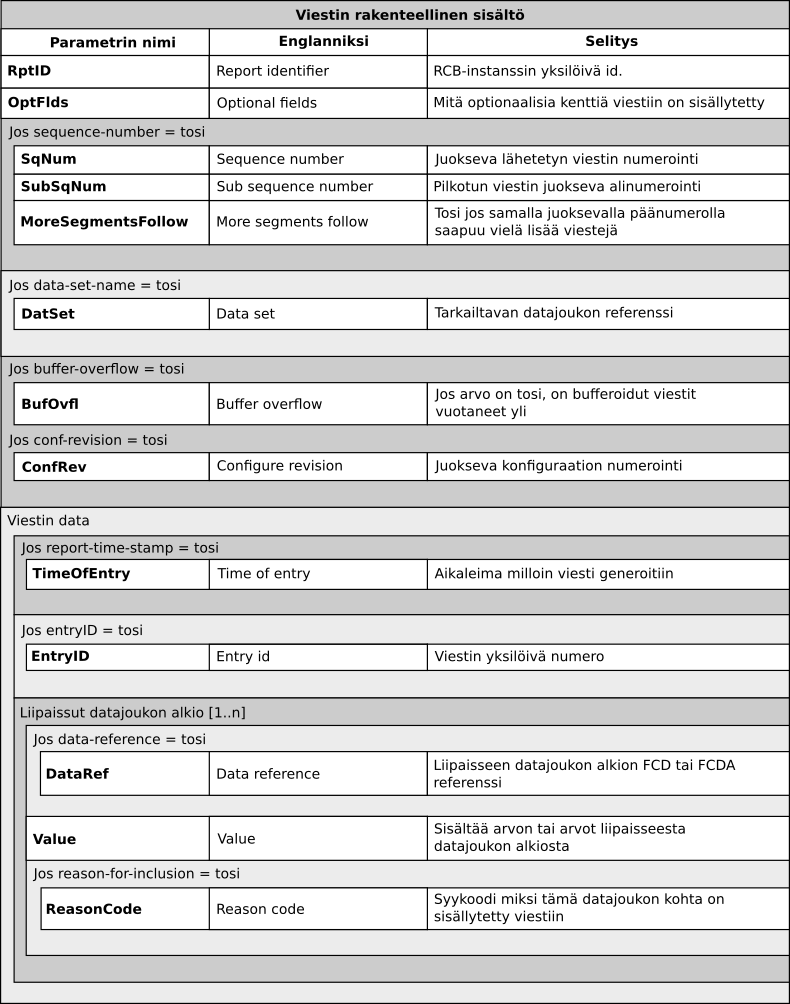
\includegraphics[width=1\textwidth]{pictures/iec61850-report-format.png}
	\caption{Standardin määrittämä lähetetyn viestin rakenne (pohjautuu kuvaan \cite[s.~104]{IEC61850-7-2}).}
	\label{fig:iec61850-report-format}
\end{figure}

Kuvassa \ref{fig:iec61850-data-set-reporting} on esitetty yleinen kuva kahden viestin lähetyksestä liipaisun tapahtuessa. Kuvassa keskellä on kaksi BRCB-instanssia myBRCB01 ja myBRCB02, jotka tarkkailevat datajoukkoja Testi1 ja Testi2 vastaavasti. Kummatkin instanssit lähettävät viestin, jotka ovat kuvassa oikealle. BRCB-instansseista voi nähdä, mitä niille asetetut attribuuttien arvot ovat ja datajoukoista näkee mistä FCD- ja FCDA -viitteistä ne koostuvat. Kuvassa attribuutin MyLD/XCBR1.Pos.stVal arvo muuttuu ja tämä liipaisee viestin lähetyksen kummassakin BRCB-instanssissa. Viesteistä voi nähdä sen sisällön ja myös miten BRCB-instanssien OptFlds-attribuutin arvot vaikuttavat sen sisältöön. Lähetettyjen viestien rakennetta ja sisältöä voi verrata kuvassa \ref{fig:iec61850-report-format} määritetyn viestin rakenteeseen. Kuvassa on esitetty myös kuinka BRCB-instansseihin viitataan MMS-protokollan tapauksessa. Tätä käsitellään tarkemmin kappaleessa \ref{ch:iec61850-mms-mallinnus}.

\begin{figure}[ht!]
	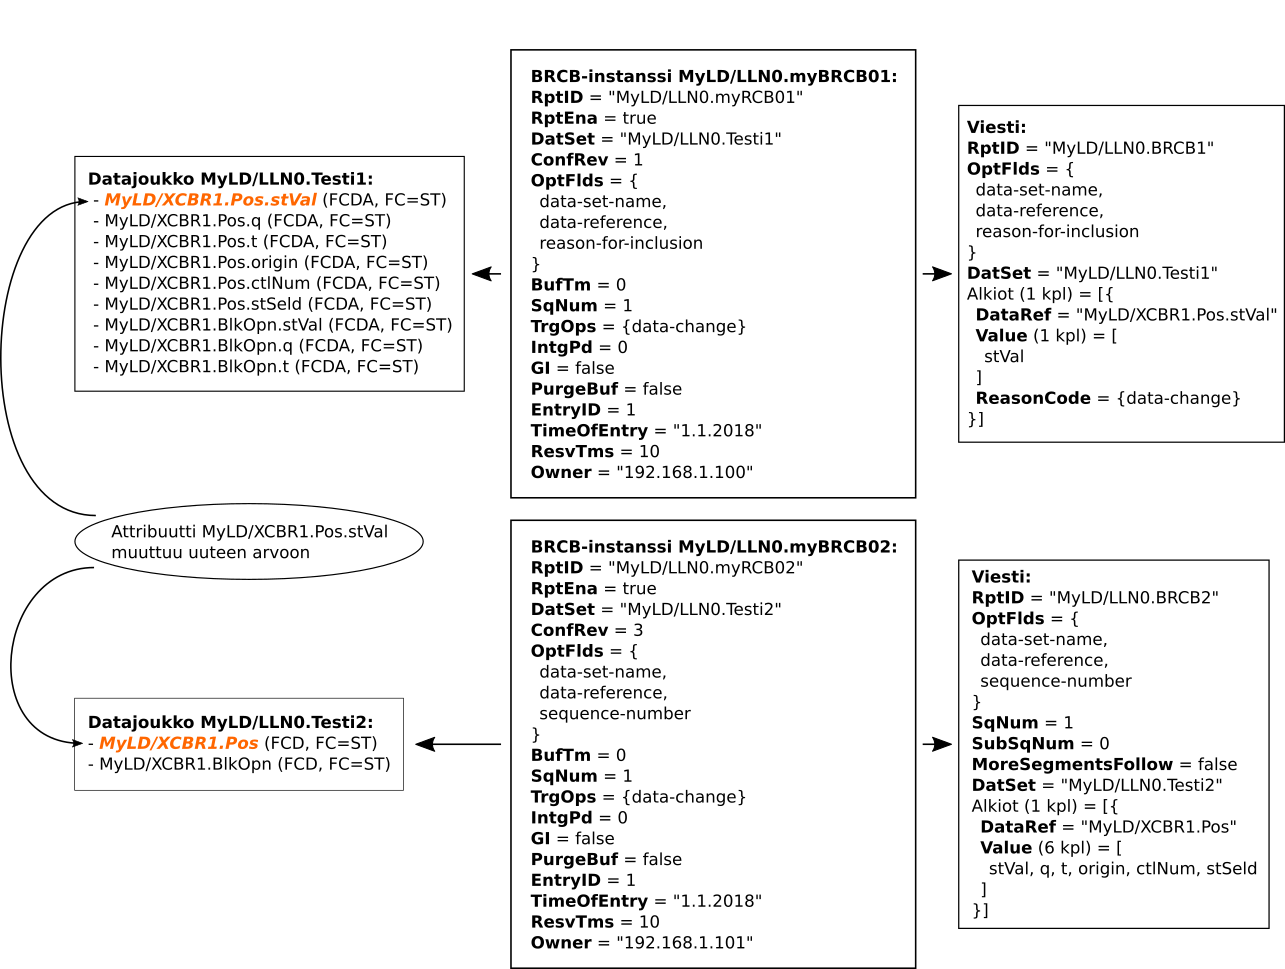
\includegraphics[width=1\textwidth]{pictures/iec61850-data-set-reporting.png}
	\caption{BRCB-instanssi tarkkailee sille määritettyä datajoukoa ja generoi viestin tapahtuman liipaistessa.}
	\label{fig:iec61850-data-set-reporting}
\end{figure}

Viestissä kenttä RptID sisältää viitteen RCB-instanssiin, mistä viestin on peräisin. OptFlds sisältää binääritietueen viestin vaihtoehtoisista kentistä. Tämä kenttä on suoraan verrattavissa viestin kenttiä SqNun, SubSqNum ja MoreSegmentsFollow käytetään kertomaan asiakkaalle, jos päätason viesti on liian pitkä ja se on pilkottu alaosiin. Kenttä SqNum on RCB-instanssin samanniminen kenttä ja on juokseva numerointi päätason viesteille. Kenttä SubSqNum on juokseva numerointi alkaen 0, jos päätason viesti, eli saman SqNum arvon sisältävä viesti on pilkottu osiin. Kentän MoreSegmentsFollow ollessa tosi asiakas tietää että päätason viesti on pilkottu osiin ja seuraava osa on odotettavissa palvelimelta. Kun viestin kaikki osat on lähetetty, palvelin asettaa viimeisessä viestissä kentän MoreSegmentsFollow arvoksi epätosi ja seuraavassa päätason viestissä SubSqNum kentän arvoksi 0. Kenttä DatSet sisältää vitteen datajoukkoon mistä viestin on peräisin. Puskuroidussa BRCB-instanssissa kenttä BufOvlf kertoo onko viestipuskuri vuotanut yli. ConfRev kertoo juoksevan konfiguraation numeron, tämä tulee suoraan RCB-instanssin samannimisestä attribuutista. TimeOfEntry kertoo milloin viesti generoitiin IED-laitteen päässä. EntryID on viestin yksilöivä numerointi. Tämä kenttä tulee suoraan RCB-instanssin samannimisestä kentästä. Tämän jälkeen viestissä tulee taulukko, joka sisältää liipaisseet datajoukon alkiot. Jokainen taulukon alkio sisältää Value-kentän ja vaihtoehtoiset DataRef ja ReasonCode kentät. DataRef sisältää datajoukon FCD- tai FCDA-viitteen, joka liipaisi tapahtuman. ReasonCode kentä kertoo mikä RCB-instanssin TrgOps-attribuutilla asetetuista liipaisimista liipaisi tapahtuman ja aiheutti alkion sisällytyksen viestiin. Kentän mahdolliset arvot ovat samat kuin RCB-instanssin TrgOps-attribuutin arvot.

Tärkeä tieto Value-kentästä on ymmärtää, että se voi sisältää yhden tai monta data-attribuutin arvoa. Tämä riippuu viittaako datajoukon liippaissut alkion FCD- vai FCDA-viitteellä kuinka moneen data-attribuuttiin. Viittauksen ollessa FCDA-viite, joka viittaa vain yhteen data-attribuutiin, sisältää Value-kenttä vain kyseisen data attribuutin arvon. Jos viittaus on FCD- tai FCDA-viite, joka viittaa moneen attribuuttiin hierarkiassa alaspäin. Sisältää Value-kenttä kaikki nämä viitatut arvot, vaikka niistä olisi liipaissut vain yksi attribuutti. FCD- ja FCDA-viittauksen toimintaa ja mitä attribuutteja se viittaa hierarkiassa alaspäin, käydään läpi kappaleessa \ref{ch:fc-and-dataset}. Esimerkki tästä on kuvassa \ref{fig:iec61850-data-set-reporting}, jossa liipaisu yhdessä attribuutissa aiheuttaa eri määrän arvoja kumpaankin viestiin. Tähän vaikuttaa kuinka liipaisevaan attribuuttiin on viitattu datajoukossa. Kuvassa datajoukossa Testi1 attribuuttiin MyLD/XCBR1.Pos.stVal on viitattu FCDA-viitteellä, jossa funktionaalinen rajoite on ST. Eli FCDA-viite viittaa vain stVal attribuuttiin, ei muihin. Tämän takia myBRCB01-instanssilta tuleva viestin Value-kenttä sisältää vain stVal-attribuutin arvon. Kun taas datajoukossa Testi2 attributtiin MyLD/XCBR1.Pos.stVal sisältyy datajoukon ensimmäiseen FCD-viitteeseen funktionaalisella rajoitteella ST. Koska FCD-viite viittaa kaikkiin Pos-instanssin alla oleviin attribuutteihin, joilla funktionaalinen rajoite on ST. Lisätään kaikki nämä attribuutit viestiin, joka lähetetään tilaajalle. BRCB-instansilta myBRCB02 tuleva viestin Value-kenttä sisältää kaikki viitatut attribuutit ja viestin DatRef-kenttä sisältää datajoukossa käytetyn viitteen. Dataobjektin Pos kaikki attribuutit voi tarkistaa taulukosta \ref{tab:iec61850-DPC-class-definition}. \cite[s.~40--44]{IEC61850-7-1} \cite[s.~108]{IEC61850-7-2}


\subsection{Abstraktimallin sovitus MMS-protokollaan}
\label{ch:iec61850-mms-mallinnus}
Tähän asti käsitellyt IEC 61850 -standardin mallit ja palvelut ovat olleet abstrahoituja ja tekniikasta riippumattomia. Tässä työssä käytetiin IEC 61850 -standardin MMS-protokollan toteutusta (engl. Manufacturing Message Specification). Tästä toteutuksesta on tarkemmin määritetty IEC 61850 -standardin osassa 8-1. MMS-protokolla on maailmanlaajuinen ISO 9506 -standardi viestintään, joka on määritetty toimivaksi TCP/IP:n pinon päällä \cite{MMS-protocol-stack-and-API}. Tämän työn kannalta lukijan ei ole tarvitse ymmärtää MMS-protokollaa ja sen toimintaa. Suunnitellussa ohjelmistossa käytettiin apuna kirjastoa, joka hoitaa matalan tason kommunikoinnin IED-laitteen kanssa. Tässä osiossa käsitellään työn kannalta tärkeitä tietoja, mitä toteutksesta MMS-protokollalle kuitenkin tarvitsee tietää. \cite{Introduction-to-the-MMS}

IEC 61850 -standardin mallinnuksessa aikaisemmin esitetty instanssien viittaus hierarkiassa muuttuu ja nyt viittaus sisältää myös funktionaalisen rajoitteen. Esimerkkinä kuvassa \ref{fig:iec61850-data-reference} oleva viite "OmaLD/Q0XCBR1.Pos.stVal" funktionaalisella rajoitteella ST, muuttuu muotoo "OmaLD/Q0XCBR1\$ST\$Pos\$stVal". Tässä viittauksessa pisteet (.) korvataan dollari-merkillä (\$). Ja kaksikirjaiminen funktionaalinen rajoite sijoitetaan loogisen noodin ja ensimmäisen data objektin nimien väliin. Muuten viittaus säilyy identtisenä alkuperäiseen ja samat rajoitteet ja nimeämiskäytännöt ovat voimassa edelleen. \cite[s.~34--35, 111]{IEC61850-8-1}

Tämän uuden viittauksen takia jokaiselle viitattavalle kohteelle täytyy olla funktionaalinen rajoite. Niinpä esimerkiksi RCB-luokkien instansseille täytyy olla myös funktionaalinen rajoite. Puskuroitua RCB-instanssia viitataan funktionaalisella rajoitteella BR. Ja puskuroimatonta funktionaalisella rajoitteella RP. Esimerkin tästä viittauksesta voi nähdä aikaisemmin mainitusta kuvasta \ref{fig:iec61850-data-set-reporting}. \cite[s.~32--34, 75]{IEC61850-8-1}


\section{Advanced Message Queuing Protocol (AMQP)}
Työssä toteutetussa ohjelmistossa IED-laitteelta verkon yli tilatut viestit ohjelma prosessoi ja lähetti viestin eteenpäin välittäjälle (engl. message broker) jonoon. Välittäjä on verkossa oleva erillinen palvelin, mistä muut ohjelmat pystyivät tilaamaan viestejä tarpeidensa mukaan. Kuvassa \ref{fig:implemented-system-communication} on esitetty lopullisen toteutuksen tietoliikenne eri osapuolten välillä. Tässä työssä toteutettu ohjelmisto on merkitty kuvaan katkoviivalla. Toteutuksessa oli kyse julkaisu ja tilaus -arkkitehtuurimallista (engl. publish-subscribe pattern), jossa työn toteutettu ohjelmisto oli tilaaja yhdeltä IED-laitteelta ja julkaisija välityspalvelimelle. Ja välityspalvelimen toisessa päässä olevat ohjelmistot olivat tilaajia. Tässä teoriaosuudessa perehdytään viestien välittäjän teoriaan, ja mitä siitä täytyy tietää ohjelmistokehityksen kannalta.

\begin{figure}[ht!]
	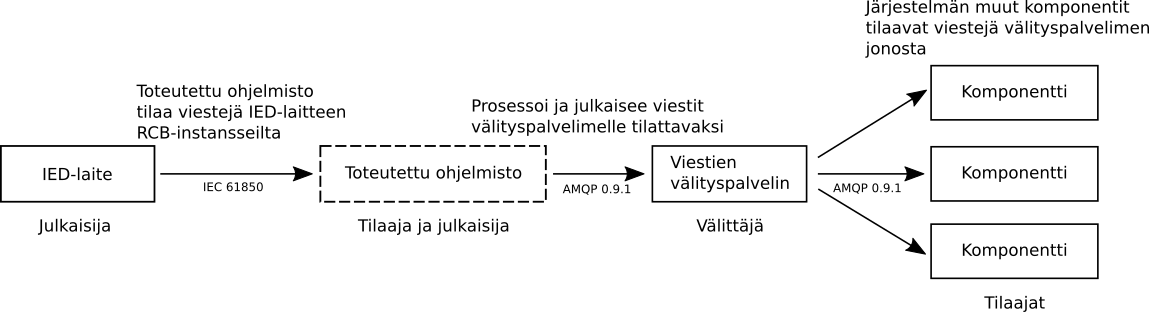
\includegraphics[width=1\textwidth]{pictures/implemented-system-communication.png}
	\caption{Toteutetun ohjelmiston osuus ja rooli käytettävässä kokonaisuudessa tietoliikenteen kannalta.}
	\label{fig:implemented-system-communication}
\end{figure}

Työssä välittäjänä käytettiin RabbitMQ-ohjelmistoa\footnote{\url{https://www.rabbitmq.com/}}, joka on avoimen lähdekoodin välittäjäpalvelin ja perustuu avoimeen AMQP-standardiin\footnote{\url{https://www.amqp.org/}} (engl. Advanced Message Queuing Protocol). AMQP määrittää yhteisen protokollan viestintään eri ohjelmistojen välillä verkon yli välityspalvelimen avulla. Verkon ansiosta välityspalvelin voi sijaita eri koneella kuin sitä käyttävät ohjelmistot. Ajan saatossa standarista on julkaistu monta eri versiota, ja työn tekohetkellä viimeisin versio oli 1.0. Kuitenkin RabbitMQ-ohjelmisto oli suunniteltu käytettäväksi suoraan standardin version 0.9.1 kanssa, ilman asennettuja lisäosia. Versioiden välinen ero oli suuri ja siirto suoraan uuteen ei olisi mahdollista, koska standardin versiot eivät olleet keskenään yhteensopivat. RabbitMQ tuki versiota 0.9.1 ja sen kehittäjät mieltävät standardin version 1.0 kokonaan eri protokollaksi \cite{RabbitMQ-Compatibility-and-Conformance}. Kuvassa \ref{fig:implemented-system-communication} on tietoliikenteen kohtiin merkitty mikä standardi vaikuttaa minkäkin osapuolen kommunikointiin. Tässä työssä välityspalvelin ja siihen yhteydessä olevat ohjelmistot käyttävät AMQP-standardista versiota 0.9.1.


\subsection{Advanced Message Queuing -malli ja sen osat}
AMQP-standardi määrittä komponentteja, joiden läpi viestin täytyy kulkea julkaisijalta tilaajalle. Standardissa nämä komponentit määrittää AMQ-malli (engl. AMQ-model). Kuvassa \ref{fig:amq-model-parts} on esitetty viestin kulku julkaisijalta tilaajalle mallin eri  komponenttien läpi. Mallin komponentit ovat \emph{vaihde} (engl. \emph{exchange}), \emph{jono} (engl. \emph{queue}) ja näiden välinen \emph{sidonta} (engl. \emph{binding}). Välityspalvelimen tehtävän voi tiivistää niin, että se ottaa vastaan viestejä julkaisijoilta vaihteeseen. Vaihde reittitää viestejä tilaajille jonoihin jonon ja vaihteen välisten sidosten mukaan. Jos tilaaja ei kerkeä prosessoida viestejä tarpeeksi nopeasti, palvelin pitää viestit jonossa tilaajelle. Vaihde voi välittää viestin moneen eri jonoon ja yhtä jonoa voi tilata monta eri asiakasta.

\begin{figure}[ht!]
	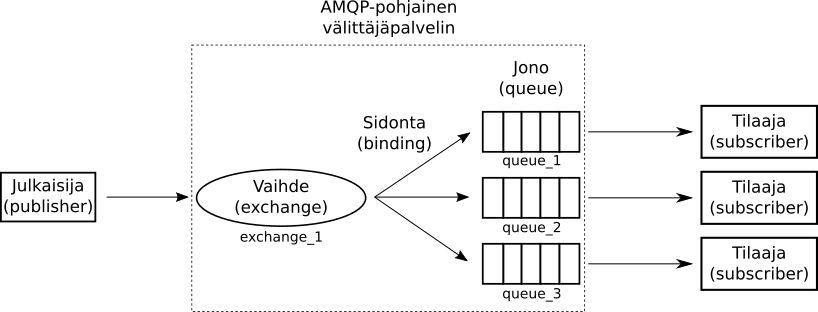
\includegraphics[width=1\textwidth]{pictures/amq-model-parts.png}
	\caption{AMQ-mallin osat ja viestin kulku niiden läpi julkaisijalta tilaajalle (pohjautuu kuvaan \cite[s.~11]{AMQP-specification}).}
	\label{fig:amq-model-parts}
\end{figure}

AMQP on ohjelmoitava protokolla siinä mielessä, että julkaisija ja tilaaja voivat määrittää komponentteja ja reitityksiä palvelimelle verkon yli ajon aikana tarpeidensa mukaan. Välittäjäpalvelin ei määritä kuin oletus vaihteet valmiiksi käytettäväksi. Eli julkaisuja voi luoda vaihteita ja tilaaja voi luoda jonoja ja sidoksia vaihdeiden ja jonojen välille. Voidaan sanoa että julkaisija ja tilaaja tekevät uusia instansseja AMQ-mallin komponenteista palvelimelle. Vaihteiden ja jonojen instansseilla täyttyy olla välityspalvelimella yksilöivät nimet, jokainen nimi asetetaan instanssin luonnin yhteydessä. Esimerkkinä kuvassa \ref{fig:amq-model-parts} on AMQ-mallin komponenttien alla niille määritetyt nimet. Vaihteella on esimerkiksi nimi exchange\_1 ja ylimmällä jonolla queue\_1. Tällä ohjelmoitavalla ominaisuudella välityspalvelin voidaan konfiguroida toteuttamaan erilaisia skenaarioita vapaasti ja se antaa kehittäjille vapautta toteutukseen.


\subsection{Vaihde (exchange) ja reititysavain (routing-key)}
Jotta viesti voidaan välittäjäpalvelimen läpi kuljettaa, täytyy julkaisijan aloittaa määrittämällä sen käyttämä vaihde (engl. exchange) ja sen tyyppi, tai käyttää palvelimen oletusvaihdetta. Vaihde on komponentti, joka ottaa vastaan viestejä ja reitittää niitä jonoihin vaihdetyypin (engl. exchange type) ja sidosten mukaan. Vaihteet eivät ikinä tallenna viestejä. Vaihde voi tiputtaa viestin, jos se ei täsmää minkään määritetyn reitityksen kanssa. AMQ-malli määrittää seuraavat käytettävät vaihdetyypit:
\begin{itemize}
	\item suoravaihde (engl. direct exchange),
	\item hajautusvaihde (engl. fanout exchange),
	\item aihepiirivaihde (engl. topic exchange) ja
	\item otsikkovaihde (engl. header exchange).
\end{itemize}

Näitä tyyppejä ja kuinka ne toimivat, käydään tarkemmin läpi tulevissa kappaleissa. Tyypin lisäksi vaihteella on myös attribuutteina nimi (engl. name), kestävyys (engl. durability), automaattinen poisto (engl. auto-delete). Nimi yksilöi vaihteen palvelimella ja tilaaja käyttää tätä nimeä sidoksen tekemiseen jonon ja vaihteen välille. AMPQ-standardissa oletetaan, että nimi on jo tiedossa etukäteen julkaisijalla ja tilaajalla. AMPQ ei tarjoa toiminnallisuutta instanssien nimien noutamiseen. Kestävyys parametrilla julkaisija voi kertoa palvelimelle, että välitäjä säilyttää vaihteen uudelleenkäynnistysten jälkeen. Jos ei, julkaisijan täytyy määrittää vaihde uudelleen käynnistyksen jälkeen. Automaattinen poisto kertoo poistaako välittäjä vaihteen automaattisesti, kun viimeinen siihen sidottu jono on poistettu ja julkaisija ei ole enää yhteydessä.

Kaikki julkaisijan ja tilaajan kutsut välittäjäpalvelimelle, jotka tekevät uuden instanssin komponentista, ovat esitteleviä (engl. declare). Tarkoittaa että palvelin tekee tarvittaessa uuden instanssin komponentista, jos sitä ei ole jo olemassa, ja vastaa samalla tavoin onnistuneesti molemmissa tapauksissa. Tilanne tulee esimerkiksi silloin kun kaksi julkaisijaa käyttävät samaa vaihdetta keskenään. Toinen ei tiedä onko toinen jo määrittänyt instanssin vaihteesta palvelimelle, esimerkiksi silloin kun ohjelmat käynnistyvät eri aikaan. Jos kummatkin julkaisijat eksplisiittisesti määrittävät saman käytettävän vaihteen. Palvelin vastaa kummallekin onnistuneesti ja tuloksena palvelimella on vain yksi instanssi halutusta vaihteesta. Sama toiminta pätee kaikkiin välittäjäpalvelimen kutsuihin, jotka tekevät uusia instansseja komponenteista.

Vaihde reitittää viestejä jonoihin sen sidosten ja tyypin mukaan. Kuitenkin reititykseen liittyy yksi tärkeä asia kuin reititysavain (engl. routing-key). Reititysavain on kuin virtuaalinen osoite viestissä, jonka julkaisija liittää viestiin julkaisun yhteydessä. Tilaaja käyttää myös reititysavainta jonon määrityksen yhteydessä. Vaihde, tyypistä riippuen, voi käyttää tätä avainta reititykseen eri jonoihin. Viestin reititysavainta voi hyvin verrata lähetettävän sähköpostin saaja-kenttään. Saaja kertoo vastaanottajan sähköpostiosoitteen, johon viesti on tarkoitus lähettää. Reititysavain toimii juurikin näin suorassa viestin lähetyksessä, mutta eroaa muissa.


\subsection{Suoravaihde (direct exchange)}
Julkaisija voi määrittää vaihteen instanssin tyypiksi suoravaihteen (engl. direct exchange). Suoravaihde reitittää viestin jonoihoin suoraan vastaavan reititysavaimen perusteella. Suoravaihde reitittää seuraavasti:
\begin{itemize}
	\item tilaaja määrittää sidoksen reititysavaimella K,
	\item julkaisija julkaisee viestin reititysavaimella R,
	\item vaihde välittää viestin jonoon jos K = R,
	\item muuten vaihde tiputtaa tai palauttaa viestin lähettäjälle.
\end{itemize}
Kuvassa \ref{fig:amqp-direct-exchange} on esitetty suoravaihteen toiminta. Vaihteeseen on tehty sidoksia reititysavaimilla \emph{error} ja \emph{info}. Yksi tilaaja voi luoda sidoksia samaan vaihteeseen monella eri reititysavaimella. Näin tilaaja voi tilata viestejä mistä on kiinnostunut. Kuvassa \ref{fig:amqp-direct-exchange} julkaisija julkaisee viestin reititysavaimella info. Viesti päätyy molempiin queue\_1 ja queue\_2 jonoon. Reititysavaimella error, viestit päätyvät vain jonoon queue\_1. Välittäjäpalvelin tarjoaa suoravaihteesta oleutusvaihteen nimeltä amq.direct. \cite[s.~27]{AMQP-specification}

\begin{figure}[ht!]
	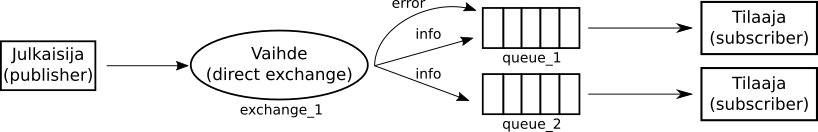
\includegraphics[width=1\textwidth]{pictures/amqp-direct-exchange.png}
	\caption{Suoravaihde (engl. direct exchange), reitittää suoraan sidoksen reititysavaimen mukaan (pohjautuu kuvaan \cite{RabbitMQ-Tutorial-Routing}).}
	\label{fig:amqp-direct-exchange}
\end{figure}


\subsection{Hajautusvaihde (fanout exchange)}
Julkaisija voi määrittää vaihteen instanssiksi hajautusvaihteen (engl. fanout exchange). Hajatusvaihde reitittää viestit kaikkiin sen jonoihin reititysavaimesta välittämättä. Hajautusvaihde toimii seuraavasti:
\begin{itemize}
	\item tilaaja määrittää sidoksen vaihteeseen reititysavaimella K,
	\item julkaisija julkaisee viestin reititysavaimella R,
	\item vaihde välittää viestin kaikkiin siihen sidottuihin jonoihin, reititysavaimesta riippumatta.
\end{itemize}
Kuvassa \ref{fig:amqp-fanout-exchange} on esitetty hajautusvaihteen toiminta. Vaihteeseen exchange\_1 on tehty kolme eri sidosta jonoihin queue\_1, queue\_2 ja queue\_3. Julkaisijan lähettämä viesti lähetetään kaikkiin kolmeen sidottuun jonoon, viestin ja jonojen reititysavaimista riippumatta. Välittäjäpalvelin tarjoaa hajautusvaihteesta oletusvaihteen nimeltä amq.fanout. \cite[s.~27]{AMQP-specification}

\begin{figure}[ht!]
	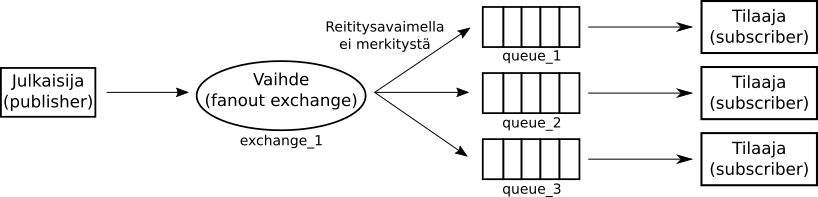
\includegraphics[width=1\textwidth]{pictures/amqp-fanout-exchange.png}
	\caption{Hajautusvaihde (engl. fanout exchange), reitittää kaikkiin siihen sidottuihin jonoihin riippumatta reititysavaimesta (pohjautuu kuvaan \cite{RabbitMQ-AMQP-0-9-1-Model-Explained}).}
	\label{fig:amqp-fanout-exchange}
\end{figure}


\subsection{Aihepiirivaihde (topic exchange)}
Aihepiiri vaihdetyyppi (engl. topic exchange) reitittää viestejä sidottuihin jonoihin reititysavaimen mukaan, kuten suoravaihde, mutta tarjoaa lisäksi sääntöjä monen avaimen samanaikaiseen yhteensopivuuteen. Sidoksen reititysavaimen sijaan voidaan puhua reitityskaavasta (engl. routing pattern). Aihepiiri vaihde toimii seuraavasti:
\begin{itemize}
	\item tilaaja määrittää sidoksen vaihteeseen reitityskaavalla P,
	\item julkaisija julkaisee viestin reititysavaimella R,
	\item vaihde välittää viestin jonoon, jos sen reitityskaava P sopii reititysavaimeen R.
\end{itemize}
Aihepiirivaihteen yhteydessä AMQP-standardi määrittää että viestin reititysavain täytyy olla lista sanoja, jotka ovat erotettu pisteillä ja maksimissaan 255 merkkiä pitkä \cite[s.~35]{AMQP-specification}. Sanat saavat sisältää kirjaimia A-Z ja a-z, ja numeroita 0-9. Yleensä avaimeen sijoitetaan sanoja mitkä liittyvät viestin sisältöön. Tilaajan määrittämä sidoksen reitityskaava voi olla samaa muotoa kuin reititysavain, mutta sanojen tilalla voidaan käyttää seuraavia erikoismerkkejä:
\begin{itemize}
	\item \textbf{*} (tähti), voi vastata mitä tahansa yhtä sanaa,
	\item \textbf{\#} (risuaita), voi vastata nolla tai monta sanaa. \cite[s.~27]{AMQP-specification}
\end{itemize}

Kuvassa \ref{fig:amqp-topic-exchange} on esitetty aihepiirivaihteen toiminta. Vaihteeseen exchange\_1 on sidottu jono queue\_1 reitityskaavoilla \textbf{app1.\#} ja \textbf{*.*.warn}. Ja jono queue\_2 reitityskaavalla \textbf{*.log.*}. Oletetaan että julkaisija lähettää viestejä avaimella muodossa \emph{ohjelma.kanava.taso}, jossa sana ohjelma kuvaa julkaisijan nimeä. Kanava, kuvaa lokitusväylää ja taso kuvaa viestin tasoa (warning, error, info jne.). Voisi sanoa että queue\_1 on kiinnostunut kaikista ohjelmalta app1 tulevista viesteistä ja myös kaikista varoitustason (warning) viesteistä kaikilta ohjelmilta. Jono queue\_2 on taas kiinnostunut kaikista log-väylän viesteistä.

\begin{figure}[ht!]
	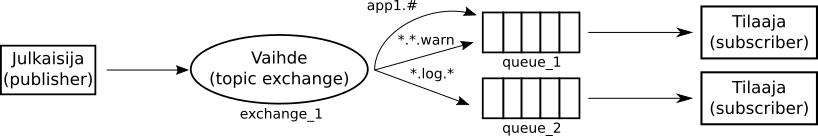
\includegraphics[width=1\textwidth]{pictures/amqp-topic-exchange.png}
	\caption{Aihepiirivaihde (engl. topic exchange), reitittää kaikkiin siihen sidottuihin jonoihin, joiden reitityskaava sopii viestin reititysavaimeen (pohjautuu kuvaan \cite{RabbitMQ-Tutorial-Topics}).}
	\label{fig:amqp-topic-exchange}
\end{figure}

Nyt jos julkaisija lähettää viestin avaimella \textbf{app1.debug.warn}. Vaihde välittää viestin jonoon queue\_1, mutta ei jonoon queue\_2. Avaimella \textbf{app2.log.info} viesti välitetään vain jonoon queue\_2. Avaimella \textbf{app1.log.warn} viesti lähetään molempiin jonoihin. Kun taas avaimella \textbf{app2.debug.info} viestiä ei lähetetä yhteenkään jonoon.

Aihepiirivaihde on vaihdetyypeistä monimutkaisin, mutta kattaa ison määrän erilaisia käyttötapauksia. Vaihteen avulla tilaajat voivat tilata viestejä, joista ovat esimerkiksi kiinnostuneita. Aihepiirivaihdetta voi käyttää kuin aikaisempia vaihdetyyppejä. Jos jono sidotaan reitityskaavalla \textbf{\#}, se vastaanottaa kaikki viestit kyseiseltä vaihteelta ja käyttäytyy kuin hajautusvaihde. Jos jono sidotaan ilman merkkejä \textbf{*} ja \textbf{\#}, niin se käyttäytyy samalla tavalla kuin suoravaihde. \cite{RabbitMQ-Tutorial-Topics}


\subsection{Otsikkovaihde (headers exchange)}
Otsikkovaihde (engl. headers exchange) on vaihdetyyppi joka ei käytä reititysavainta ollenkaan reititykseen, vaan reititys perustuu viestin ja sidoksen otsikkotietoihin. Otsikkotiedot koostuvat avain--arvo-pareista. Otsikkovaihde toimii seuraavasti:
\begin{itemize}
	\item tilaaja määrittää sidoksen vaihteeseen otsikkotiedoilla H,
	\item julkaisija julkaisee viestin otsikkotiedoilla O,
	\item vaihe välittää viestin jonoon jos otsikkotiedot O vastaavat otsikkotietoja H, riippuen sidoksen otsikkotiedoissa olevasta \textbf{x-match} kentän arvosta.
\end{itemize}
Jonon sidoksen määrityksen yhteydessä tilaaja voi asettaa kentän \textbf{x-match} otsikkotietoihin ja sille arvon kahdesta eri mahdollisuudesta \textbf{all} tai \textbf{any}. Arvot toimivat seuraavasti:
\begin{itemize}
	\item \textbf{all} kertoo vaihteelle, että jokainen viestin otsikkotieto täytyy vastata sidoksen otsikkotietoja (boolen algebrassa AND-operaatio), jotta viestin lähetetään jonoon,
	\item \textbf{any} kertoo vaihteelle, että mikä vain viestin otsikkotiedoista löytyy sidoksen otsikkotiedoista (boolen algebrassa OR-operaatio), lähetetään viesti jonoon. \cite[s.~28]{AMQP-specification}
\end{itemize}

Otsikkotiedoissa arvot ovat vaihtoehtoisia asettaa. Jos kentän arvoa ei ole asetettu, vastaavuus on kun kentän nimet ovat samat. Jos kentän arvo on asetettu, vastaavuus on jos molemmat nimi ja arvo vastaavat toisiaan. \cite[s.~28]{AMQP-specification}


\subsection{Jonon määritys ja viestien kuittaaminen}
AMQ-mallissa jono (engl. queue) on vaihteen ja tilaajan välissä oleva puskuri (kuva \ref{fig:amq-model-parts}), joka tallentaa tilaajalle tulevia viestejä. Jono pitää viestejä jonossa tilaajelle, kunnes tämä kerkiää prosessoida ne. Yksi jono voi puskuroida viestejä monelle eri tilaajalle. Tilaaja sitoo (engl. binding) jonon nimellä johonkin palvelimelle jo olevaan vaihteeseen mistä viestejä haluaa. Tilaajan täytyy tietää vaihteen nimi jo etukäteen. Jonolla tilaaja voi määrittää attribuutteja. Jotkin attribuutit ovat samoja kuin vaihteella. Tilaaja voi määrittää jonolle nimen (engl. name), kestävä (engl. durable), eksklusiivinen (engl. exclusive) ja automaattinen poisto (auto-delete). Nimi yksilöi jonon palvelimella. Tilaaja voi halutessaan pyytää palvelinta generoimaan yksilöivän nimen jonolle automaattisesti. Kestävyys säilyttää jonon palvelimella uudelleenkäynnistyksen jälkeen. Eksklusiivinen rajoittaa jonon vain yhdelle tilaajalle, ja palvelin poistaa jonon kun yhteys tilaajaan katkeaa. Automaattinen poisto poistaa jonon palvelimelta automaattisesti, kunnes yhteys viimeiseen tilaajan on katkennut. \cite{RabbitMQ-AMQP-0-9-1-Model-Explained}

Jono lähettää viestin vain yhdelle jonossa olevalle tilaajalle. Sama viesti lähetetään ainoastaan toiselle tilaajalle, jos se edelleenlähetetään virheen tai peruutuksen seurauksena. Jos samassa jonossa on monta eri tilaajaja, jono lähettää viestejä monelle tilaajalle kiertovuorottelun (engl. round-robin) periaatteen mukaan. \cite[s.~11--12]{AMQP-specification}

Tilaajan täytyy määrittä jonolle sen käyttämä viestin kuittaamisen (engl. acknowledge) malli, ennen kuin jono poistaa viestin puskurista. Malleja on kaksi:
\begin{itemize}
	\item automaattinen, jolloin palvelin poistaa viestin jonosta heti kun se on lähetetty tilaajalle,
	\item eksplisiittinen, jolloin palvelin poistaa viestin vasta kun tilaaja on lähettänyt kuittauksen palvelimelle.
\end{itemize}
Tilaaja voi lähettää viestistä kuittauksen milloin vain prosessoinnin aikana. Heti kun viesti on vastaanotettu, tai silloin kun viesti on prosessoitu. \cite[s.~29]{AMQP-specification}



















